%% This is an example first chapter.  You should put chapter/appendix that you
%% write into a separate file, and add a line \include{yourfilename} to
%% main.tex, where `yourfilename.tex' is the name of the chapter/appendix file.
%% You can process specific files by typing their names in at the 
%% \files=
%% prompt when you run the file main.tex through LaTeX.

\chapter{Variability in the mechanisms controlling Southern Ocean phytoplankton bloom phenology in an ocean model and satellite observations
}
\label{chap:2}
\raggedbottom

{\let\thefootnote\relax\footnotetext{This chapter was originally published as Rohr, T.R., Long, M.C., Kavanaugh, M.T., Lindsay, K., Doney, S.C. (2017). \href{https://doi.org/10.1002/2016GB005615}{Variability in the mechanisms controlling Southern Ocean phytoplankton bloom phenology in an ocean model and satellite observations.} \emph{Global Biogeochemical Cycles} 31: 922-40. }}

{\let\thefootnote\relax\footnotetext{T.R. conducted analysis and wrote the manuscript with input from all authors.}}
%{\let\thefootnote\relax\footnotetext{The supplemental methods, figures, and tables for this chapter can be found in \cref{sec:app2}.}}

\clearpage


%%%%%%%%%%%%%%%%%
\section{Abstract}

A coupled global numerical simulation (conducted with the Community Earth System Model) is used in conjunction with satellite remote sensing observations to examine the role of top-down (grazing pressure) and bottom-up (light, nutrients) controls on marine phytoplankton bloom dynamics in the Southern Ocean. Phytoplankton seasonal phenology is evaluated in the context of the recently proposed `disturbance-recovery' hypothesis relative to more traditional, exclusively `bottom-up' frameworks. All blooms occur when phytoplankton division rates exceed loss rates to permit sustained net population growth, however the nature of this decoupling period varies regionally in CESM. Regional case studies illustrate how unique pathways allow blooms to emerge despite very poor division rates or very strong grazing rates.  In the Subantarctic, southeast Pacific small spring blooms initiate early co-occurring with deep mixing and low division rates, consistent with the `disturbance-recovery' hypothesis. Similar systematics are present in the Subantarctic, southwest Atlantic during the spring, but are eclipsed by a subsequent, larger summer bloom that is coincident with shallow mixing and the annual maximum in division rates, consistent with a `bottom-up', light limited framework. In the model simulation, increased iron stress prevents a similar summer bloom in the southeast Pacific. In the simulated Antarctic zone (70$^{\circ}$S - 65$^{\circ}$S) seasonal sea ice acts as a dominant phytoplankton-zooplankton decoupling agent, triggering a delayed but substantial bloom as ice recedes. Satellite ocean color remote sensing and ocean physical reanalysis products do not precisely match model predicted phenology, but observed patterns do indicate regional variability in mechanism across the Atlantic and Pacific. 

%%%%%%%%%%%%%%%%%
\section{Introduction}

Southern Ocean (SO) net community production (NCP) and the associated `biological pump' play a critical role in oceanic carbon storage [e.g., \textcite{MarinovImpactoceaniccirculation2008}; \textcite{HauckSouthernOceanCO22015}], carbon cycling \parencite{SiegelGlobalassessmentocean2014} and thus global climate dynamics \parencite{ChisholmOceanographyStirringtimes2000,TreguerPrefaceClimaticchanges2002}. In the SO, iron limitation \parencite{MartinIrondeficiencylimits1990,BoydEnvironmentalFactorsControlling2002}, seasonal sea ice cover \parencite{ArrigoSeculartrendsArctic2011} and trophic dynamics constrain the net population growth of phytoplankton to seasonal blooms \parencite{LonghurstEcologicalGeographySea2006}. Understanding these seasonal cycles in phytoplankton ecosystem dynamics is critical to our understanding of spatial and temporal variability in Southern Ocean NCP but is hampered by the complexity of interconnected physical, chemical, and biological controls. 

Phytoplankton bloom dynamics are governed by bottom-up factors that control cell division rates, as well as top-down factors that control grazing and other loss rates. The net effect on seasonal net population growth is a balance between a number of different, and often opposing, bottom-up and top-down factors, and as a result, the timing of bloom initiation can vary substantially geographically and from year to year. 

From a bottom-up perspective, light limitation can suppress division rates during deep winter mixing when depth averaged photosynthetically active radiation (PAR) over the mixed layer is low. For a bloom to occur, the springtime mixed layer depth must shoal above some critical level for depth-averaged PAR to drive levels of community photosynthesis above losses \parencite{GranQuantitativeStudyPhytoplankton1935, RileyFactorsControllingPhytoplankton1946, SverdrupConditionsVernalBlooming1953}. In this context, phytoplankton biomass concentration is assumed to be well coupled to the depth-integrated inventory, and bloom initiation is typically estimated as the point in time when surface concentrations begin to increase substantially \parencite{SiegelNorthAtlanticSpring2002}. However, some observations indicate that depth integrated biomass can increase before the mixed layer shoaled above this critical depth \parencite{TownsendSpringphytoplanktonblooms1992, EllertsenSpringbloomsstratification1993, DaleSeasonaldevelopmentphytoplankton1999} implying that bloom inception may be influenced by other mechanisms including dilution (or disturbance)-recovery \parencite{FischerSixtyYearsSverdrup2014}. 

Mixed layer deepening can mediate `top-down' controls on bloom development \parencite{BehrenfeldAbandoningSverdrupCritical2010,BehrenfeldAnnualcyclesecological2013} and decouple concentration-based and inventory-based growth rates. Bloom initiation, instead defined as the switch to positive net growth of the column-integrated population rather than surface concentration, can be triggered by subtle disequilibria in trophic coupling that decrease predation by zooplankton and promote sustained increases in phytoplankton biomass integrated over the mixed layer. This disequilibrium is modulated, in part, by entrainment during the fall and winter of phytoplankton depleted water during deep mixing, diluting the phytoplankton concentration on which grazing rates depend. Since grazing scales with prey concentrations, dilution can cause loss rates to drop below division rates; thus, deep mixing can actually maintain (or increase) the vertically integrated phytoplankton inventory \parencite{BehrenfeldAbandoningSverdrupCritical2010,BehrenfeldAnnualcyclesecological2013}. Under this `disturbance-recovery' framework, bloom initiation can occur even while phytoplankton cell division rates are deteriorating (i.e., via increased light limitation from mixed layer deepening) so long as loss rates are declining at a faster rate (i.e., via dilution effects on predation).

From a bottom-up perspective, deep mixing can also entrain nutrients from depth, replenishing surface levels of macro- and micronutrients \parencite{CarranzaSouthernOceanwinddriven2015}, which are known to limit net primary productivity \parencite{MooreProcessespatternsoceanic2013}. In particular, throughout the Southern Ocean, iron is largely thought to be the dominant limiting nutrient, leading to expansive High Nitrate, Low Chlorophyll (HNLC) regions \parencite{MartinIrondeficiencylimits1990, deBaarImportanceironplankton1995, deBaarSynthesisironfertilization2005, Boydbiogeochemicalcycleiron2010}. However, the degree of iron limitation across the Southern Ocean is quite variable in space and time. Regional inputs from atmospheric dust deposition, anoxic coastal sediments, river runoff, and sea/glacial ice provide exogenous iron sources of varying significance \parencite{MooreSedimentarymineraldust2008,BoydMappingphytoplanktoniron2012} that can modify bloom size and duration, and regulate the importance of deep mixing as an iron source. 

Sea ice can both hinder high latitude bloom development through severe surface light limitation \parencite{ArrigoSeculartrendsArctic2011} and support cell division following ice melt via increased vertical stratification \parencite{SmithPhytoplanktonbloomproduced1985,SmithInfluenceseaice2008} and nutrient enrichment (particularly Fe) \parencite{SedwickRegulationalgalblooms1997, FennelImpactsironcontrol2003, LancelotSpatialdistributioniron2009}. Note, however, nutrient enrichment from ice melt is not incorporated into many global-scale ocean biogeochemical models including the one used in this analysis (see \textbf{section 3.2}). As Southern Ocean sea-ice dynamics are modified by climate change \parencite{StammerjohnRegionsrapidsea2012} these competing processes can lead to dramatically different effects on bloom dynamics. Depending on regional wind conditions and total ice concentration, decreased sea ice could dampen or amplify the bloom 
\parencite{Montes-HugoRecentchangesphytoplankton2009}. 

This complex suite of controls drives variability in the size \parencite{SullivanDistributionsphytoplanktonblooms1993, MoorePhytoplanktonchlorophylldistributions2000} and timing \parencite{RacaultPhytoplanktonphenologyglobal2012, ThomallaRegionalscalecharacteristics2011} of phytoplankton blooms, which can affect trophic transfer and carbon export. Disentangling these controls is critical in understanding present, and predicting future, spatio-temporal variability in Southern Ocean NCP, and ultimately the role of marine autotrophs in a changing climate. In this study, model results and remote sensing observations are used to showcase how physical and biogeochemical controls can produce blooms via different mechanisms. In doing so, we test the suitability of the `disturbance-recovery' hypothesis relative to more traditional, strictly `bottom-up' systematics.

We first highlight the observed and simulated spatial variability in bloom size and timing across the Southern Ocean (see \textbf{section 4.1.1}). Next we analyze how well coupled peak cell division rates are to peak net population growth rates and peak biomass inventory within the model to help infer the strength of bottom-up controls (see \textbf{section 4.1.2}). Different mechanistic pathways are then explicitly examined by comparing the simulated climatologies of the relevant physics and biogeochemistry for four spatially averaged regional case studies simulated in CESM (see \textbf{section 4.2}). Finally, the two model regions with the most dramatic differences and most complete remote sensing coverage are compared to the observations (see \textbf{section 4.3}).  


%%%%%%%%%%%%%%%%%
\section{Methods}

%%%%%%%%%%%%%%%%%
\subsection{Numerical Experiments}

The Community Earth System Model (CESM) is a fully coupled, global climate model capable of simulating past, present, and future climate scenarios \parencite{HurrellCommunityEarthSystem2013}. Here we utilize a preindustrial simulation with a recently improved treatment of photosynthesis under sea ice \parencite{LongModelingphotosynthesissea2015}. The new treatment better represents the effect of subgrid-scale heterogeneity in sea-ice thickness and water column irradiance on the non-linear (concave downward \parencite{Geiderdynamicregulatorymodel1998}) photosynthesis-irradiance curve, leading to a more realistic phenology and bloom magnitude. This 30-year simulation has been branched off a longer control simulation, and most model output was saved at high temporal resolution as daily means. 

Except for the new sea-ice treatment, the component set up is identical to that of the 1850 control used in the CESM Large Ensemble project and described in detail by \textcite{KayCommunityEarthSystem2014}. The ocean component has nominal horizontal resolution of 1 degree and 10m vertical grid cells down to $250m$. Sea ice is treated using the CICE4 component \parencite{HunkeCICEAlamosSea2008}. The ice model does not sequester iron or resolve any biogeochemistry. All atmospheric dust deposition over sea ice is deposited directly into the surface water.  
The ocean biogeochemistry component (BEC) detailed by \parencite{MooreMarineEcosystemDynamics2013} has been tested and validated against global datasets and shown to capture basin-scale spatial distributions in production, nutrient and chlorophyll concentrations 
\parencite{DoneySkillmetricsconfronting2009g, MooreUpperoceanecosystem2004,MooreMarineEcosystemDynamics2013,MooreProcessespatternsoceanic2013}, and key aspects of oceanic iron \parencite{MooreSedimentarymineraldust2008} and carbon cycling \parencite{LimaDynamicsparticulateorganic2014, LongTwentiethCenturyOceanicCarbon2013,MooreMarineEcosystemDynamics2013}. BEC features a single class of zooplankton and three phytoplankton functional types: diatoms, small phytoplankton, and diazotrophs. Diazotrophs, however, are strongly limited by temperature and therefore exist only in negligible concentrations in the Southern Ocean. Phaeocystis, which have been observed to dominate coastal, SO blooms \parencite{SchoemannPhaeocystisbloomsglobal2005}, are not resolved but are unlikely to outcompete diatoms in the iron depleted simulated open ocean due to lower iron uptake efficiency \parencite{WangIncorporatingPhaeocystisSouthern2011a}. Phytoplankton carbon biomass, $C_{phyto} (mmol \: C)$, is tracked in terms of grid cell concentration, $[C_{phyto}] (mmol \quad C \quad m^{-3})$. Phytoplankton net population growth $(\frac{d[C_{phyot}]}{dt})$ is governed by a photosynthetic net primary productivity term, $P_{phyto}$, and opposed by losses due to a grazing, $G_{phyto}$, linear mortality, $mort_{phyto}$, and quadratic mortality/aggregation, $agg_{phyto}$, term, such that,

\begin{equation}
    \frac{d[C_{phyto}]}{dt} = P_{phyto}-G_{phyto}-mort_{phyto}-agg_{phyto},
\end{equation}

\noindent{where all terms are in $(\frac{mmol  \: C} {m^{3} \: d^{1}})$ and phyto represents either of the two regionally dominant pools of autotrophic plankton resolved in the simulation, diatoms or small phytoplankton.}

Grid cell net primary productivity $(P_{phyto})$ is equal to a volumetric specific photosynthetic division rate, $\mu (d^{-1})$, multiplied by the biomass concentration $(P_{phyto} = \mu[C_{phyto}])$. The specific photosynthetic division rate is subject to temperature dependence ($L^T$), multi-nutrient ($N, P, Si, Fe$) limitation ($L^n$) and light availability ($L^{I_{PAR}}$). Individual nutrient limitation terms vary from 0 to 1 as a nonlinear function of the available nutrient concentration and a class-specific nutrient specific half saturation coefficient. Multi-nutrient limitation is treated following Liebig's Law of the minimum \parencite{vanderPloegOriginTheoryMineral1999} such that the maximum specific photosynthetic division rate ($\mu^{max}_{phyto}$) is only scaled by the most limiting nutrient limitation term rather than a multiplicative function of each. Note that because the nutrient limitation term scales the maximum growth rate lower values translate to greater nutrient stress.  Nutrient stress is systematically less for small phytoplankton than for diatoms given the same nutrient concentration because of differences in the parameterization of their respective half saturation coefficients chosen to account for differences in their size and physiology \parencite{SundaIronuptakegrowth1995}. Light limitation ($L^{I_{PAR}}$) scales as a nonlinear function of photosynthetically available radiation, a dynamic $Chl:C$ ratio and the most constraining nutrient limitation term. Both the $Chl:C$ ratio and nutrient limitation terms are computed differentially for individual phytoplankton pools resulting in a species specific light limitation term. Together,

\begin{equation}
    \mu = \mu^{max}_{phyto} L^T l^n L^{I_{PAR}}.
\end{equation}

Grazing occurs on individual phytoplankton pools and is governed by a temperature dependent, non-linear function (Holling type II; \parencite{HollingCharacteristicsSimpleTypes1959}) of the phytoplankton concentration such that,

\begin{equation}
    G_{phyto} = \mu^{max}_{zoo;phyto} L^T (\frac{[C_{phyto}]^2}{[C_{phyto}]^2 +g^2_{phyto}}) [Z_C],
\end{equation}

\noindent{where $\mu^{max}_{zoo;phyto}  (d^{-1})$ is the maximum zooplankton specific grazing rate on phytoplankton class $phyto$, $L^T$ is the dimensionless temperature dependency term, $[C_{phyto}]$ is the class-specific phytoplankton carbon concentration $(mmol \: C \: m^{-3})$, $g_{phyto}$ is the zooplankton class-specific grazing coefficient ($mmol \: C \: m^{-3}$), and $[Z_C]$ is the zooplankton carbon biomass concentration ($mmol \: C \:  m^{-3}$). The class specification of the grazing parameterization ensures that zooplankton are more effective grazers on the small phytoplankton class, affording a relatively complex trophic control on phytoplankton at an affordable computational cost. Zooplankton is in turn governed by differential grazing on all three phytoplankton populations weighted by a non-dimensional ingestion coefficient and a temperature dependent loss term. The nonlinearities of the grazing equation ensure that zooplankton become more efficient grazers as phytoplankton concentrations increase, eventually saturating towards a maximum grazing rate.}


%%%%%%%%%%%%%%%%%
\subsection{Remote sensing and reanalysis data}

We analyze ocean color remote sensing records compiled at 8-day resolution from 2005-2014 from the MODIS/Aqua satellite program. Observational indicators of phytoplankton abundance and growth include MODIS surface chlorophyll records, as well as phytoplankton carbon biomass and cell division rates estimated from particle backscattering and absorption coefficients using the GSM spectral matching algorithm \parencite{GarverInherentopticalproperty1997} and the carbon based productivity model (CbPM) outlined by \textcite{BehrenfeldCarbonbasedoceanproductivity2005} and later improved and validated against global datasets by \textcite{WestberryCarbonbasedprimaryproductivity2008}. Observationally-based mixed layer depth estimates are sourced from HYCOM and FNMOC reanalysis projects \parencite{MilutinovicSensitivityremotesensing2009}. HYCOM and FNMOC data sets are merged for improved spatial and temporal coverage. All aforementioned data has been sourced from the Oregon State Ocean Productivity webpage \parencite{OMalleyOceanproductivity2015}. Daily sea-ice fractional coverage is estimated at $25km$ resolution using the GSFC Bootstrap SMMR-SSM/I Version 2 time series \parencite{ComisoPassivemicrowavealgorithms1997, ShangComparisonprimaryproductivity2010,ComisoLargeDecadalDecline2011}.

%%%%%%%%%%%%%%%%%
\subsection{Quantification of relevant rates and metrics}

%%%%%%%%%%%%%%%%%
\subsubsection{Phytoplankton metrics}

All modeled phytoplankton metrics (unless otherwise noted) are calculated for the sum of the two regionally dominant phytoplankton functional types, small phytoplankton and diatoms (See \textbf{section 3.1}). CESM resolves both and carbon and chlorophyll concentrations for each phyotoplakton pool using a dynamic Chl:C ratio to account for photoacclimation. In our analysis, phytoplankton abundance is quantified in carbon units. Daily modeled and observed $[Chl_{phyto}]_{surf}$ values are used in our diagnostic analysis to approximate the euphotic depth following the empirical relationship developed by \parencite{MorelSurfacepigmentsalgal1989}. In the prognostic simulation, the full chlorophyll profile is used to calculate light penetration, however only surface chlorophyll concentrations ($[Chl_{phyto}]_{surf}$) are saved at daily-mean resolution.

Model simulated, depth resolved profiles of $[C_{phyto}]$ were only saved as monthly means, and therefore exact values of phytoplankton carbon inventory ($\Sigma C_{phyto}$) integrated to time-varying mixed layer depth or euphotic depth can only be computed from monthly averages of biomass and depth. However, daily-mean simulated values are available for the phytoplankton carbon inventory integrated over the upper $100m$ of the water column ( $\Sigma C^{100}_{phyto}, \: mmol \: C \: m^{-2}$). Assumptions regarding the vertical distribution of biomass allow us to approximate both daily total water column inventory and surface concentrations. Following \textcite{BehrenfeldAnnualcyclesecological2013}, we assume that phytoplankton biomass is homogenously distributed across the greater of the mixed layer depth or euphotic depth ($Z_{eu}$), referred to as the $Profile \: Depth$, $Z_{profile} = max(MLD, Z_{eu})$. Biomass is assumed to drop to 0 below this depth. This assumption holds well for an actively mixing mixed layer that is deeper than the euphotic depth, though could be problematic for shallow mixed layers where phytoplankton biomass can persist in stratified water below the mixed layer depth \parencite{BossObservationspigmentparticle2008, Bosssituevaluationinitiation2010,BehrenfeldAnnualcyclesecological2013} or when there is little active mixing [Franks et al., 2015]. Specifically in the Southern Ocean, \parencite{UitzVerticaldistributionphytoplankton2006} concluded from in-situ data sets that it was reasonable to assume a uniform distribution in deep, well-mixed water.

The water column phytoplankton carbon inventory is thus assumed equal to the vertical integral over $Z_{profile}$ ($\Sigma C_{phyto} = \int^{Z^{profile}}_{surface} [C_{phyto}] dZ, \; mmol \: C \: m^{-2}$). For the model analysis, we use the daily-mean $100m$ integral to approximate the inventory ($\Sigma C_{phyto} = \Sigma C^{100}_{phyto}$) when $Z_{profile} < 100m$, recognizing that non-zero biomass in the depth range $Z_{profile}-100m$ may violate our distribution assumption; however this assumption does not bias our approximation of total water column inventory. Additional biomass below $100m$ is unaccounted for but unlikely to be significant given a shallow $Z_{profile}$. When $Z_{profile} > 100m$ we extrapolate from $100m$ to $Z_{profile}$ using the mean $0-100m$ concentration ($\Sigma C_{phyto} = (\frac{Z_{profile}}{100}\Sigma C^{100}_{phyto})$). Here the assumption of a uniform profile is reasonable, particularly in CESM, given a deep, well-mixed layer that likely exceeds the euphotic depth.  

Modeled surface carbon biomass concentrations ($[C_{phyto}]_{surf}, \: mmol \: C \: m^{-3}$) also were saved only as monthly means. Daily surface concentrations are first approximated by assuming a uniform depth profile across $Z_{profile}$ and dividing inventory by profile depth ($[C_{phyto}]_{surf} = \Sigma C_{phyto}/Z_{profile}$ ). This approximation can be problematic for shallow mixed layers where biomass may exist in the euphotic zone below the mixed layer depth. To improve our first approximation for shallow profiles ($Z_{profile}<100m$), estimated surface concentrations are further weighted by a spatially and profile depth dependent correction factor modeled from the simulated monthly surface concentration data (see \textbf{appendix A2.1}). Testing the skill of this approach with the monthly data demonstrated a strong match between the corrected approximate surface concentrations and true-modeled values across the Southern Ocean (see \textbf{A2.1}).

Remote sensing observations provide only surface concentrations, which are extrapolated to $Z_{profile}$ following \parencite{BehrenfeldAnnualcyclesecological2013}, under the same uniform depth distribution assumption.

Volumetric phytoplankton specific net population growth rates, $r$ ($d^{-1}$), can be related to the specific photosynthetic division rate, $\mu$ ($d^{-1}$), by 

\begin{equation}
    \frac{1}{[C_{phyto}]} \frac{d[C_{phyto}]}{dt} = r=y-l,
\end{equation}

\noindent{where $l \: (d^{-1})$ is the total specific loss rate composed of grazing ($l_{G,}_{phyto}$) , phytoplankton mortality ($l_{mort,}_{phyto}$), and aggregation ($l_{agg,}_{phyto}$) (see Eq. 2.1). Volumetric specific rate terms ($\mu, \: l$) for a grid cell are calculated by normalizing the rate terms as they appear in Eq. 2.1 by the biomass concentration ($\mu = \frac{P_{phyto}}{[C_{phyto}]}$; $l = \frac{l_{G,phyto}+l_{mort,phyto}+l_{agg,phyto}}{[C_{phyto}]}$)}

Population specific rates for the vertically-integrated population ($ \mu_{\Sigma}$, $l_{\Sigma G,phyto}$, $l_{\Sigma mort,phyto}$, $l_{\Sigma agg,phyto}$; $d^{-1}$) are calculated by dividing the water column integrated daily rate terms ($\Sigma P_{phyto}$, $\Sigma G_{phyto}$, $\Sigma mort_{phyto}$, $\Sigma agg_{phyto}$; $mmol \: C \: m^{-2} d^{-1}$) by the depth integrated phytoplankton carbon inventory ($\Sigma C_{phyto}$). The total population specific loss rate ($l_{\Sigma}$) is the sum of its components ($l_{\Sigma} = l_{\Sigma G,}_{phyto} + l_{\Sigma mort,phyto} + l_{\Sigma agg,phyto} $).

In the model, rate terms ($P_{phyto},G_{phyto},mort_{phyto},agg_{phyto}$) are saved as daily mean $150m$ depth resolved profiles. If $Z_{profile}>150m$, we assume that $rates(z>150m) = rates(z=150m)$.The population specific net growth rate for the depth-integrated inventory, $r_{\Sigma}$  ($d^{-1}$), can thus be explicitly calculated as

\begin{equation}
    r_{\Sigma} = u_{\Sigma} - l_{\Sigma}
\end{equation}

Without explicitly resolved rate terms, in the remote sensing data $r_{\Sigma}$  ($d^{-1}$), between two time points, t=0 and t=1, is calculated from temporal changes in phytoplankton biomass as follows,

\begin{equation}
    r_{\Sigma} = ln (\Sigma C_{phyto-1}/\Sigma C_{phyto-0})/\Delta t, \textrm{if MLD is deepening and }> Z_{eu}
\end{equation}
\begin{equation}
    r_{\Sigma} = ln ([C_{phyto-1}]_{surf}/[C_{phyto-0}]_{surf})/\Delta t, \textrm{ if MLD is shoaling or }< Z_{eu}
\end{equation}

\noindent{where either concentration or vertical inventory is used, depending on mixed layer dynamics, to take into account dilution effects by entrainment of phytoplankton free water from below during deep mixed layer deepening. Bloom initiation is in turn defined as the onset of positive population net growth rates, $r_{\Sigma} > 0$. A more comprehensive explanation can be found in \parencite{BehrenfeldAbandoningSverdrupCritical2010, BehrenfeldAnnualcyclesecological2013}. Note, the model $r_{\Sigma}$ as derived diagnostically from the simulation (Eq. 2.5) is able to explicitly isolate only biogeochemical factors (division and loss terms); however the formulation for the remote sensing data (Eq. 2.6) implicitly assigns all changes in population size to biological factors and thus neglects contributions from physical transport terms. Spatially averaged regional binning in \textbf{section 4.2} should, however, largely average out the effect of physical processes in the remote sensing data.}

All nutrient and light limitation terms are explicitly resolved in the model and saved as daily mean depth profiles down to $150m$. Mean community representative limitation terms are averaged over the $Z_{profile}$. Consistent with the rate term depth profiles, the deepest saved limitation term is extrapolated to depth if $Z_{profile}>150m$. 

%%%%%%%%%%%%%%%%%
\subsubsection{Sea-ice metrics}

The day of sea-ice retreat in a grid cell is defined as the day fractional ice coverage falls below 15\% [e.g. \parencite{StammerjohnTrendsAntarcticannual2008}] and remains below this threshold for at least 30 days; if this condition is not met, there is considered to be no retreat for that grid cell in that year. Alternatively, if annual ice does not exceed 15\% fractional coverage for at least 50 days there is considered no advance. Interannual correlations calculated with the day of retreat only consider years with a well-defined retreat date and grid cells with a minimum of ten such years.  

%%%%%%%%%%%%%%%%%
\subsection{Model Skill Metrics}

CESM solutions are compared to observational values inferred from the remote sensing/reanalysis products. Various metrics are used to test model skill and are computed independently at each grid cell between 45\degree S and 55\degree S. Ice coverage and higher solar zenith angles at higher latitudes lead to unsatisfactory seasonal remote sensing coverage relative to the lower latitudes. The model error is computed as the root mean square deviation of CESM and observational climatologies normalized by the observed maximum. The model peak magnitude/timing biases are computed as the difference between the maxima of CESM and observed climatologies. The peak magnitude bias is further normalized by the observed climatological maximum. Positive(negative) biases mean the model magnitude is over(under) estimated and timing is delayed(early). Correlation coefficients between CESM and observed climatologic time series are computed at each grid cell with zero lag. Metrics are reported as spatial averages and `circumpolar' values refer to the mean of all grid cells between 45S\degree and 55S\degree.

%%%%%%%%%%%%%%%%%
\subsection{Regional Bins}

We focus on the dynamics of four regionally averaged case studies chosen to provide explicit examples of some of the variability in bloom structure and mechanism simulated and observed in the Southern Ocean. All reported metrics are computed first at individual grid cells prior to spatial averaging. We examine a zonal comparison between the temperate SE Pacific (Bin P1: 55\degree S - 45\degree S, 100\degree W-80\degree W) and SW Atlantic (Bin A1: 55\degree S - 45\degree S, 60\degree W-40\degree W) as well as a latitudinal progression from the temperate SE Pacific though the sub-polar SE Pacific into the seasonal sea-ice zone (Bins P1, P2: 65\degree S -55\degree S, 100\degree W-80\degree W, and P3: 70\degree S -65\degree S, 100\degree W-80\degree W, respectively). All four regional bins are outlined in \textbf{Fig. 1 \& 2}. Our selection is justified in \textbf{Sec. 2.3.3} in the context of results from \textbf{2.4.1} and \textbf{2.4.2}. 

%%%%%%%%%%%%%%%%%
\section{Results}

%%%%%%%%%%%%%%%%%
\subsection{Large-scale Southern Ocean patterns}

%%%%%%%%%%%%%%%%%
\subsubsection{Peak bloom size and timing}

Southern Ocean distributions of remotely sensed (\textbf{Fig. 1a}) and model simulated (\textbf{Fig. 1c}) maximum $[C_{phyto}]_{surf}$ display some important qualitative similarities. Both showcase dramatic spatial variability in bloom magnitude and a notable increase in peak $[C_{phyto}]_{surf}$  moving poleward, along regions of coastal upwelling, and in the southwest Atlantic basin (\textbf{Fig. 1a, c}). Quantitatively, the circumpolar model error is 66\%. The CESM biomass maxima are systematically too high, with a circumpolar peak magnitude bias of 143\%, and miss some smaller scale spatial structure likely related to mesoscale features of the Antarctic Circumpolar Current. In particular, the model error is worst in the SW Atlantic (180\% in Bin A1, see \textbf{Fig. 1}), however the amplification of the SW Atlantic basin relative to the SE Pacific is coherent between the simulation and observations. Accordingly, we focus here on qualitative differences in bloom development as opposed to absolute magnitudes, addressing these quantitative discrepancies further in \textbf{Sec. 2.4.3}.

Spatial variability is also apparent in peak bloom timing, with peak $[C_{phyto}]_{surf}$  generally occurring later at higher latitudes in both observations (\textbf{Fig. 1b}) and the simulation (\textbf{Fig. 1d}). However, the model predicts substantially earlier maxima in the open ocean than the observations. In particular, blooms in the SE Pacific (Bin P1 in \textbf{Fig. 1}) are biased by -53 days. The implications of this discrepancy in the context of bloom mechanics are also addressed in \textbf{Sec. 2.4.3}.  

Depth integrated inventories provide a valuable, complementary picture of bloom dynamics. The circumpolar model error for  $\ΣC_{phyto}$ is 38\%. In both model and observations (see \textbf{Sec. 2.4.3}) simulated peak $\ΣC_{phyto}$ does not necessarily align with the size or timing of peak $[C_{phyto}]_{surf}$. Notably, in the model many open-ocean regions exhibit peak $\ΣC_{phyto}$ prior to peak $[C_{phyto}]_{surf}$ (e.g. $\sim3$ weeks earlier in Bin P1 - \textbf{Fig. 1d, f}), while in the sea-ice zone (black contour - \textbf{Fig. 1-3}) and parts of the SW Atlantic the peaks co-occur. While a larger magnitude of peak $[C_{phyto}]_{surf}$ typically corresponds with larger peaks in inventory, closer examination reveals this relationship is not linear. The ratio of peak($\ΣC_{phyto}$):peak($[C_{phyto}]_{surf}$) is highly variable, ranging from $10-30$ m in the SW Atlantic (e.g. Bin A1) to upwards of 100 m in the SE Pacific (e.g. Bin P1) despite similar mean peak mixing depths between A1 ($156m$) and P1 ($164m$) indicating differences in timing and/or mechanism. 

%%%%%%%%%%%%%%%%%
\subsubsection{Cell Division and Net Population Growth Rates}

Variability in the simulated co-evolution of cell division and net population growth rates reveals implicit differences in the underlying mechanisms controlling the variability in simulated bloom phenology displayed in \textbf{Fig. 1}. In a theoretically idealized system completely controlled from the bottom-up, population specific loss rates would be invariant in time and all variability in $r_\Sigma$ would be described by $\mu_\Sigma$. \textbf{Fig. 2}, however, shows a large degree of variability in the degree of coherence between $\mu_\Sigma$ and $r_\Sigma$ across the SO in CESM suggesting that a variety of different mechanisms control net population growth ($r_\Sigma$). 

In the SW Atlantic (in particular Bin A1) $r_\Sigma$ peaks just before peak $\mu_\Sigma$ (\textbf{Fig. 2c}), when $\mu_\Sigma$ exceeds 80\% of the annual maximum (\textbf{Fig. 2a}). Following peak $\mu_\Sigma$ and $r_\Sigma$, biomass continues to accumulate for weeks (\textbf{Fig. 2d}) until $\mu_\Sigma$ drops below $\sim$50\% of the annual maximum (\textbf{Fig. 2b}), finally receding below $l_\Sigma$ and terminating the bloom. This is consistent with a strong bottom-up control in which $r_\Sigma$ and $\mu_\Sigma$ tend to co-vary. 

Similarly, in the seasonally ice-covered region (\textbf{Fig. 2} - 30\% mean annual ice contour; Bin P3 - \textbf{Fig. 2}) peak $r_\Sigma$ and $\mu_\Sigma$ are well aligned (\textbf{Fig. 2a,c}). However, peak $\ΣC_{phyto}$ occurs while $\mu_\Sigma$ is still quite high (~>70\% of annual maximum – \textbf{Fig 2b}) indicating the stronger role of increasing loss rates and top-down controls in bloom shut down, opposed to $\mu_\Sigma$ simply receding below less variable $l_\Sigma$.

In contrast over much of the simulated open Southern Ocean, and in particular Bin P1, peak $r_\Sigma$  (\textbf{Fig. 2c}) and $\ΣC_{phyto}$ (\textbf{Fig. 2d}) occur in quick succession when ~<50\% of annual maximum and months before peak $\mu_\Sigma$ . It follows that peak $r_\Sigma$ can be, but is not always, largely decoupled from the strict evolution of cell division rates – a direct reflection of bottom-up growth conditions. The decoupling of $r_\Sigma$ and $\mu_\Sigma$ emphasizes the importance of temporally variable loss rates and top-down controls.

%%%%%%%%%%%%%%%%%
\subsection{CESM Regional Case Studies: Zonal and Latitudinal Comparisons}

We highlight the explicit climatologies of several of the qualitatively different mechanisms implied in \textbf{Fig. 2}. Four regional case studies are chosen on the basis of 1. Providing a zonal comparison and latitudinal gradient, 2. Exhibiting strong variability in bloom size and timing in the simulation and observations (see \textbf{Fig. 1}), 3. Exhibiting strong variability in the simulated coherence between  and  (see \textbf{Fig. 2}), 4. Highlighting two mechanistic pathways subject to debate in the current literature (The Critical Depth and Disturbance-Recovery Hypotheses) and 5. Falling in proximity to two Ocean Observatory Initiative (OOI) sampling sites to enable the possibility of future in-situ comparisons. 

%%%%%%%%%%%%%%%%%
\subsubsection{Zonal Comparison: Temperate, Open-Ocean SE Pacific (Bin P1) vs. Temperate, Open-ocean SW Atlantic (Bin A1)}

The simulated temperate SE Pacific (P1) and SW Atlantic (A1) bins exhibit similar spring bloom dynamics. In both regions, a small spring bloom with localized peak $\Sigma C_{phyto}$ occurs in October after a positive division-loss decoupling ($r_\Sigma > 0$, \textbf{Fig. 3d}; $\mu_\Sigma > l_\Sigma$, \textbf{Fig. 4a, b}) in September. The early spring decoupling is coincident with the period of maximum deep mixing and strong light limitation (\textbf{Fig. 4 c,d}). Despite favorable iron availability (relative to the annual cycle), phytoplankton division rates are flat or even deteriorating during bloom initiation and remain low and only slightly improving throughout the decoupling period (\textbf{Fig. 4}).  

The behavior of the regions diverges over the late spring and summer, with much larger Atlantic $[C_{phyto}]_{surf}$ (\textbf{Fig. 3c}) and  (\textbf{Fig. 3e}). These summertime biomass differences arise despite broadly similar patterns of seasonal mixing (\textbf{Fig. 3a}) and $\mu_\Sigma$ (\textbf{Fig. 3f}) and reflect the cumulative effect of a second positive division-loss decoupling during November and December in the Atlantic ($r_\Sigma>0$, \textbf{Fig. 3d}; $\mu_\Sigma > l_\Sigma$, \textbf{Fig. 4b}) versus more closely coupled conditions in the Pacific ($r_\Sigma \sim 0$, \textbf{Fig. 3d}; $\mu_\Sigma \sim l_\Sigma$, \textbf{Fig. 4a}). The regional variations may arise because the Atlantic bin experiences weaker spring-early summer iron limitation (\textbf{Fig. 4c, d}) and thus elevated $\mu_\Sigma$ during shoaling (\textbf{Fig. 3c}; \textbf{Fig. 4a, b}). Division rates eventually fall back below declining loss rates by early January in part because of self-shading and elevated light limitation (\textbf{Fig. 4d}) leading to bloom termination ($r_\Sigma < 0$, Fig. 3d;$\mu_\Sigma < l_\Sigma$, \textbf{Fig. 4b}) 


%%%%%%%%%%%%%%%%%
\subsubsection{Latitudinal Progression: Sub-polar SE Pacific (Bin P2) \& Seasonal Ice Zone SE Pacific (Bin P3)}

Peak and annual mean  progressively deteriorate poleward (from P1 to P3; \textbf{Fig. 5f}) due to colder temperatures and stronger annual mean light limitation (\textbf{Fig. 4d}, \textbf{Fig. 6c,d}) caused by the combined effects of weakening incoming solar irradiation, deeper mixing (P2) and/or seasonal sea-ice coverage (P3). Despite worsening cell division conditions, peak $\Sigma C_{phyto}$  increases at higher latitudes (from P1 to either P2 or P3) due to significantly longer and larger decoupling periods ($r_\Sigma>0$; $\mu_\Sigma \> l_\Sigma$). In the sub-polar SE Pacific (P2) the sizable spring decoupling period is qualitatively similar to that of P1 but notably longer, allowing  to continue to slightly outpace $l_\Sigma$ through December (\textbf{Fig 6a}). Although the sub-polar SE Pacific bloom peaks in early summer when division rates are high (like A1), it is initiated while cell division conditions are poor and eventually shutdown by increasing grazing rates opposed to deteriorating division rates (like P1).

In the higher latitudes (Bin P3, \textbf{Fig. 5}; \textbf{Fig. 6}) seasonal sea-ice coverage drives division (and in turn grazing) rates towards zero during the winter leading to standing phytoplankton stocks lower than in other bins. As ice recedes, improved surface PAR is accompanied by a rapidly shoaling mixed layer stabilized by fresh melt water input, together acting to improve light availability. Grazing rates (hampered by a small initial zooplankton population) lag significantly behind the surge in division rates (\textbf{Fig. 6c}) leading to a long decoupling period and the largest sustained population specific net growth rates of any analyzed bin. The bloom culminates in the largest peak $\Sigma C_{phyto}$ and $[C_{phyto}]_{surf}$ of all Pacific bins before grazing rates rebound and surpass division rates just prior to optimal division rates (\textbf{Fig. 6b}).

%%%%%%%%%%%%%%%%%
\subsection{Remote Sensing/Reanalysis Zonal Comparison}

The CESM simulation allows for the exploration of possible mechanisms decoupling division and loss rates to permit a bloom, but does not necessarily imply that these mechanisms are representative of dynamics in the real ocean in these specific regions. It is informative, therefore, to compare the regional variability between bin P1 and A1 in the model to that of the observations (\textbf{Fig. 7}) in a mechanistic context.

The model error in Bin P1, A1 and the complete circumpolar band is respectively 31\%, 21\% and 27\% for $MLD$; 21\%, 86\% and 38\% for $\Sigma C_{phyto}$; 20\%, 180\% and 66\% for $[C_{phyto}]_{surf}$; 30\%, 44\% and 35\% for $r_\Sigma$; 25\%, 35\% and 35\% for $\mu_\Sigma$. The correlation coefficient between CESM and observed climatologies averaged over A1 and P1 is .86 for $MLD$, .52 for $[C_{phyto}]_{surf}$, and .45 for $\Sigma C_{phyto}$. Model error is significant, but within the observed range, and despite high frequency variability of the relevant processes, CESM is able to capture some of the variability in important state variable at a fine daily resolution.

The largest model-data discrepancies in our regional analysis are in the bloom phenology of the temperate SE Pacific (Bin P1) and bloom magnitude of temperate SW Atlantic (Bin A1). In the temperate SE Pacific (P1), model $[C_{phyto}]_{surf}$ peak much earlier than in the observations (-64 day bias). Model $\Sigma C_{phyto}$ also peaks earlier than observations, but less so (-22 day bias). This can likely be attributed to discrepancies in simulated mixing dynamics, which resolve a shallower maxima (-43\% bias) and earlier minimum (-34 day bias); other physical factors, such as incident $PAR$ and $SST$ seasonal climatologies, are generally consistent between model and observations for P1 and A1 bins. Nevertheless, the mechanisms seem to align: peak inventory occurs while mixing is deeper and is followed by a delayed peak in concentration once mixing shoals. 

In the temperate SW Atlantic (A1) the phenology of the summer $\Sigma C_{phyto}$ bloom is well aligned (-13 day bias); however the peak magnitude is much larger in the model (201\% bias). Interestingly though, this overshoot occurs despite dramatically higher observed division rates, implicitly necessitating much higher loss rates as well.

Discrepancies not-withstanding, some important similarities in the relative phenology and magnitude of P1 and A1 underscore the variability in mechanism seen in CESM. In both the observations and the simulation, the temperate SE Pacific (P1) has a larger ratio of peak $\Sigma C_{phyto}$ to peak $[C_{phyto}]_{surf}$ (\textbf{Fig. 7e,c}) than the temperate SW Atlantic (A1). Observations agree that the bloom is much closer to the mixing maxima and further from optimal division rates ($\mu_\Sigma$ in P1 than in A1; Averaged over all observed individual years and relevant grid cells, peak $\Sigma C_{phyto}$ is 48 days closer to peak mixing and 32 days further from peak $\mu_\Sigma$ in P1 than A1. 

Finally, observations show implicit evidence of a dynamic loss term supplementing bottom-up processes as a critical control on biomass. Cell division rates are only 9\% (in P1) and 12\% (in A1) of their annual maximum during observed peak net population growth, implicitly requiring loss rates to be acting as an important control. 


%%%%%%%%%%%%%%%%%
\section{Discussion}

The seasonal accumulation of depth-integrated biomass, referred to as a bloom, is ultimately dependent on a disequilibrium between cell division rates and loss rates. As many physical and biogeochemical factors interact to regulate a bloom, multiple mechanistic pathways can theoretically affect the magnitude, duration, and phasing of decoupling throughout the course of the year. Simulations, supported by observational indicators, illustrate variability in the type of mechanistic pathways possible throughout the SO.   

The frequency distributions of $\frac{\mu_\Sigma \textrm{at peak} r_\Sigma}{\textrm{peak} \mu_\Sigma}$ for all CESM SO grid cells (\textbf{Fig. 8}) reveals a wide range over which the delicate balance between $\mu_\Sigma$ and $l_\Sigma$ can yield peak net population growth rates – not just when $\mu_\Sigma$ is climaxing or $l_\Sigma$ is bottoming out as a singularly bottom-up or top-down paradigm would predict. 

Case studies were selected to explicitly examine contrasting regional dynamics, but are not intended to precisely prescribe the entire set of SO dynamics. Our selection of open-ocean bins does however provide a diverse sample of the overall distribution (\textbf{Fig. 8}); The mean $\frac{\mu_\Sigma \textrm{at peak} r_\Sigma}{\textrm{peak} \mu_\Sigma}$ across our regional bins is 1.4 standard deviations below (P1), 1.6 standard deviations above (A1), and within .1 standard deviation (P2) of the distribution mean. P3 falls near the mean ($\sim .3$ standard deviations) of the distribution of ice covered grid cells. Practical considerations to omit in depth climatological analysis from the rest of the SO leave open the possibility of regions exhibiting dynamics distinct from those presented; however, this would only strengthen our argument that variable pathways can control bloom phenology. 

In all open ocean bins (P1, P2, \& A1), CESM simulates an early spring bloom that initiates amidst poor cell division conditions and terminates while division rates are still improving. This early season bloom is concurrent with deep mixing and driven by a dilution-decoupling mechanism. In the North Atlantic, \textcite{BehrenfeldAnnualcyclesecological2013} attributed strong positive interannual correlations between peak phytoplankton inventory and peak mixing depths in both observations and simulations as evidence of dilution-driven trophic decoupling. The same correlation computed from our model run across the Southern Ocean (\textbf{Fig. 9a}) implies that this mechanism is prevalent but does not dominate everywhere within the model domain. A strong positive correlation is found in P1 and P2 where the seasonal cycle is limited to a single, dilution driven bloom. In P2, where the correlation is slightly higher, a longer and larger deep mixing period (relative to P1) increases the magnitude of initial decoupling, thereby yielding a longer and larger early bloom, even as the mixed layer proceeds to shoal (\textbf{Fig. 5}; \textbf{Fig. 6}). The entrainment of nutrient rich deep water \parencite{CarranzaSouthernOceanwinddriven2015} and subsequent reduction of iron stress (\textbf{Fig. 4c}) helps bolsters very low, light-limited division rates (\textbf{Fig. 4a}), and sustains this decoupling period from the bottom-up; however, the disparity between $\mu_\Sigma$ and  $r_\Sigma$ necessitates the critical role of dilution effects. Most regions displaying a strong positive correlation between deep mixing and peak biomass (\textbf{Fig. 9a}) also overcome low cell division rates during peak net population growth (\textbf{Fig. 2a}) implying dilution driven processes are relevant elsewhere throughout the Southern Ocean.

In the A1 region of CESM, the correlation between peak inventory and mixing is notably weaker than in the Pacific sector; indeed, the simulation shows negative correlation in places (\textbf{Fig. 8a}) because a second, dominant summer bloom effectively overwhelms the contribution of the local dilution-driven spring bloom to the annual signal. This larger bloom initiates amidst favorable cell division conditions and does not shut down until cell division rates are in decline. It is concurrent with shallow mixing and resembles a more traditional, bottom-up, light limited bloom. Despite a disproportionate increase in summertime biomass the absolute magnitude of $\mu_\Sigma$ is only slightly elevated relative to P1 (a 3\% increase in the annual peak and 7\% increase in the annual mean – see \textbf{Fig. 4a}), necessitating the additional role for variable trophic interactions in distinguishing A1 and P1. The emergence of this summer bloom in the A1 region relative to P1 is attributed to a greater supply of iron which elevates division rates just enough to remain slightly decoupled from grazing during the light-favorable, shallow summer mixing period. 

Both modeling \parencite{Misumiironbudgetocean2014} and observational \parencite{TagliabueSurfacewaterironsupplies2014} studies have found vertical mixing to be the dominant supply mechanism of new iron into the euphotic zone in the Southern Ocean. However, episodic iron inputs from atmospheric deposition \parencite{GaieroIronothertransition2003} and heterogeneous sedimentary fluxes that supplement deep-water iron stocks \parencite{MooreSedimentarymineraldust2008,TagliabueEvaluatingimportanceatmospheric2009} contribute to regional variability in iron availability. Bin A1 experiences strong exogenous sources of iron relative to the Pacific from both seafloor sediments and aeolian dust deposition in nature \parencite{GaieroIronothertransition2003, MooreSedimentarymineraldust2008, TagliabueEvaluatingimportanceatmospheric2009} and in the CESM. As a result, modeled iron limitation is consistently reduced in the Atlantic relative to the Pacific, with the most severe seasonal iron stress in A1 (\textbf{Fig. 4d} - black traces) being quantitatively on par with the most growth-conducive iron conditions in P1 (\textbf{Fig. 4c}). Reduced iron stress in Bin A1 keeps division rates slightly higher than in P1 during mixed layer shoaling, compensating for increasing self-shading and grazing as a large summer bloom accumulates in A1 but is absent in P1. 

Transitioning in CESM from the perennially open ocean to the seasonally ice covered Antarctic zone, the distribution of $\frac{\mu_\Sigma \textrm{at peak} r_\Sigma}{\textrm{peak} \mu_\Sigma}$ (see \textbf{Fig. 8}) has a much smaller range than in the open-ocean and is skewed toward higher values, indicative of a stronger bottom-up forcing driven by seasonal sea ice. In the simulated SE Pacific (bin P3) bloom phenology is more in phase with ice than mixing dynamics. There is a clear mechanistic pathway for seasonal sea ice to first suppress a bloom – via light limitation - before triggering a bloom during retreat - via relieved light limitation, melt water input, water column restratification, and potential trophic decoupling. \textbf{Figure 9b} shows the interannual correlation between the day of ice retreat and peak bloom inventory. The correlation changes from positive (i.e. a longer ice season correlating a with larger peak bloom) at low latitudes in the marginal ice zone to strongly negative further south, suggesting a shift in the balance between the dominance of the suppression and stimulation pathways. A similar latitudinal transition was observed by \textcite{Montes-HugoRecentchangesphytoplankton2009} along the Western Antarctic Peninsula, where declining sea-ice severity has led to opposite ecosystem responses in the north (smaller blooms) and the south (larger blooms).  

Significant bias and error exist in both the remote sensing data and model output. Both the model and observations have a relatively coarse resolution that may average out more intricate ecosystem dynamics. Passive remote sensing data are forced to interpolate over cloud-covered days and reflect only daytime values. SO remote sensing is particularly challenging, with biases associated with ice, solar angle, seasonal coverage and changes in particle size distribution \parencite{DierssenBioopticalpropertiesremote2000}. Further, data are subject to the many assumptions implicit in the NPP and biomass algorithms \parencite{BehrenfeldCarbonbasedoceanproductivity2005, WestberryCarbonbasedprimaryproductivity2008, BehrenfeldAnnualcyclesecological2013}. 

Model solutions are of course limited by computational constraints on the number of processes and constituents that can be resolved and the uncertainty associated with the complexity and parameterization of those that are. In particular, CESM lumps all zooplankton species into a single pool and underestimates SO winter mixing depths \parencite{MooreMarineEcosystemDynamics2013}. Both could account for the discrepancies between observed and simulated bloom timing (P1) and magnitude (A1) seen in \textbf{Sec. 2.4.3}. Feedbacks within over-simplified food webs could alter the timing of trophic interactions, while the mixing bias could decrease the flux of deep nutrients, permit higher concentrations of overwintering zooplankton, and relax community light limitation \parencite{DoneySkillmetricsconfronting2009g}. Such simplifications can certainly influence phytoplankton division and population growth rates, limiting the ability of CESM to precisely predict robust regional estimates of $NPP$.

Nevertheless, simulated division and population growth rates fall within range of those observed experimentally in the SO. Division rates derived from a variety of techniques (e.g. radiotracers, direct cell counts, etc.) ranged from roughly .1 to 1 ($d^{-1}$) \parencite{SakshaugPhotoadaptationAntarcticphytopfankton1986,SpiesGrowthratesAntarctic1987,SmithPhytoplanktongrowthrates1999}. Net population growth rates measured by \textcite{BoydControlphytoplanktongrowth2001} were roughly an order of magnitude smaller and ranged from -.05 to .1 ($d^{-1}$).

Further, confidence in the qualitative nature of simulated bio-physical interactions (e.g. the grazing functional form \parencite{Fashamnitrogenbasedmodelplankton1990, Doneynewcoupledonedimensional1996}, species specific grazing rates, species specific light \parencite{Geiderdynamicregulatorymodel1998} and nutrient \parencite{vanderPloegOriginTheoryMineral1999} limitation) insulate our more general qualitative conclusions about how bottom-up and top-down controls can respond to environmental forcing to yield a bloom in different ways. While our results may not offer a precise map of where mechanistic differences emerge in nature, they do provide a theoretical underpinning of how and why mechanisms may diverge across the Southern Ocean.

Despite significant quantitative disagreements, qualitative observational indicators in the remote sensing data support the model finding of regional variability in the mechanisms controlling bloom phenology. In the SE Pacific, observations and simulation agree that peak biomass in the temperate SE Pacific occurs much closer to the mixing maxima and cell division rate minimum than in the temperate SW Atlantic, where biomass inventory does not peak until cell division rates are much higher, and closer to their annual maximum, highlighting the significance of both top-down and bottom-up controls and strengthening the veracity of theoretical differences in how and why blooms can form. This message is not intended to diminish the importance of bottom up controls but rather to caution against neglecting the other term in the equation: $r_\Sigma =\mu_\Sigma - l_\Sigma$.

Disentangling the role of these competing rate terms will prove only more important as climate change alters the landscape of the SO. In an intermodel comparison study \parencite{LaufkotterDriversuncertaintiesfuture2015} found that 4 of 9 models predicted decreasing $NPP$ under RCP 8.5 despite improving division rates resulting from declining biomass driven by stronger grazing rates. In turn, \textcite{LaufkotterDriversuncertaintiesfuture2015} stress the need to better understand the phenological and trophic coupling mismatches that can regulate phytoplankton biomass (and thus $NPP$) from the top down. Moving forward it is important to not only better understand these mechanisms but to understand which environmental landscapes support them, otherwise we risk making qualitatively backwards assumptions about the effect climate change will have on net community production.  


%%%%%%%%%%%%%%%%%
\section{Conclusions}

Throughout the simulated Southern Ocean we observe several distinct mechanistic pathways underlying the spatial variability in bloom phenology, supported by indicators in the observational record. While bottom-up factors are clearly important, discrepancies in the seasonal evolution of division rates and net population growth rates in model and observations stress the equally important role of temporally varying loss rates. Both bottom-up and top-down controls play a significant, but variable role, with some blooms climaxing amidst annually optimal cell division rates and other amidst very poor cell division rates but even weaker grazing rates. 

The `disturbance-recovery' hypothesis [Behrenfeld et al., 2013] examined in the North Atlantic certainly appears relevant in the simulated Southern Ocean as well. In all CESM case study regions, population specific loss rates and division rates co-vary for much of the year; Periods of subtle disequilibria permit positive net population growth rates that are typically an order of magnitude lower than either the growth or loss terms. The dilution-recoupling mechanism looks to be prevalent during deep mixing in the simulated open ocean, however it is evident that other mechanistic decoupling pathways exist as well.

Despite some discrepancies between model and observations, there is ample and coherent evidence to support the notion that blooms can form via several distinct pathways across the Southern Ocean. Still, because results derive largely from a single model integration it is important to focus not on precisely where certain mechanisms emerge but rather on the theoretical implications of how these different pathways can inform the role of SO biogeochemistry in a changing climate. We hope this work will encourage other modeling groups to examine more carefully the biophysical mechanisms governing seasonal phenology and to routinely archive key model metrics at the required higher temporal resolution.

\subsubsection{Acknowledgements}
The CESM project is supported by the National Science Foundation and the Office of Science (BER) of the U.S. Department of Energy. Computing resources were provided by the Climate Simulation Laboratory at NCAR’s Computational and Information Systems Laboratory (CISL), sponsored by the National Science Foundation and other agencies. This research was enabled by CISL compute and storage resources. TR was supported by an NDSEG graduate fellowship. SCD and  MTK acknowledge support from the National Aeronautics and Space Administration Ocean Biology and Biogeochemistry Program (NNX14AL86G) and the National Science Foundation Polar Programs award 1440435 (Antarctic Integrated System Science) to the Palmer LTER program. Please contact trohr@mit.edu for further questions or to access to data. 





%%%%%%%%%%%%%%%%%%%%%%%%%%%%%%%%%%%%%%%%%%
        %%     Figures  %%
%%%%%%%%%%%%%%%%%%%%%%%%%%%%%%%%%%%%%%%%%%



%%%%%%%%%%%%%%%%%%%%%%%%
%%%%%% Figure 1 %%%%%%%%
%%%%%%%%%%%%%%%%%%%%%%%%

\begin{figure}[!htbp]
\begin{adjustwidth}{-1in}{-1in}
 \centering
 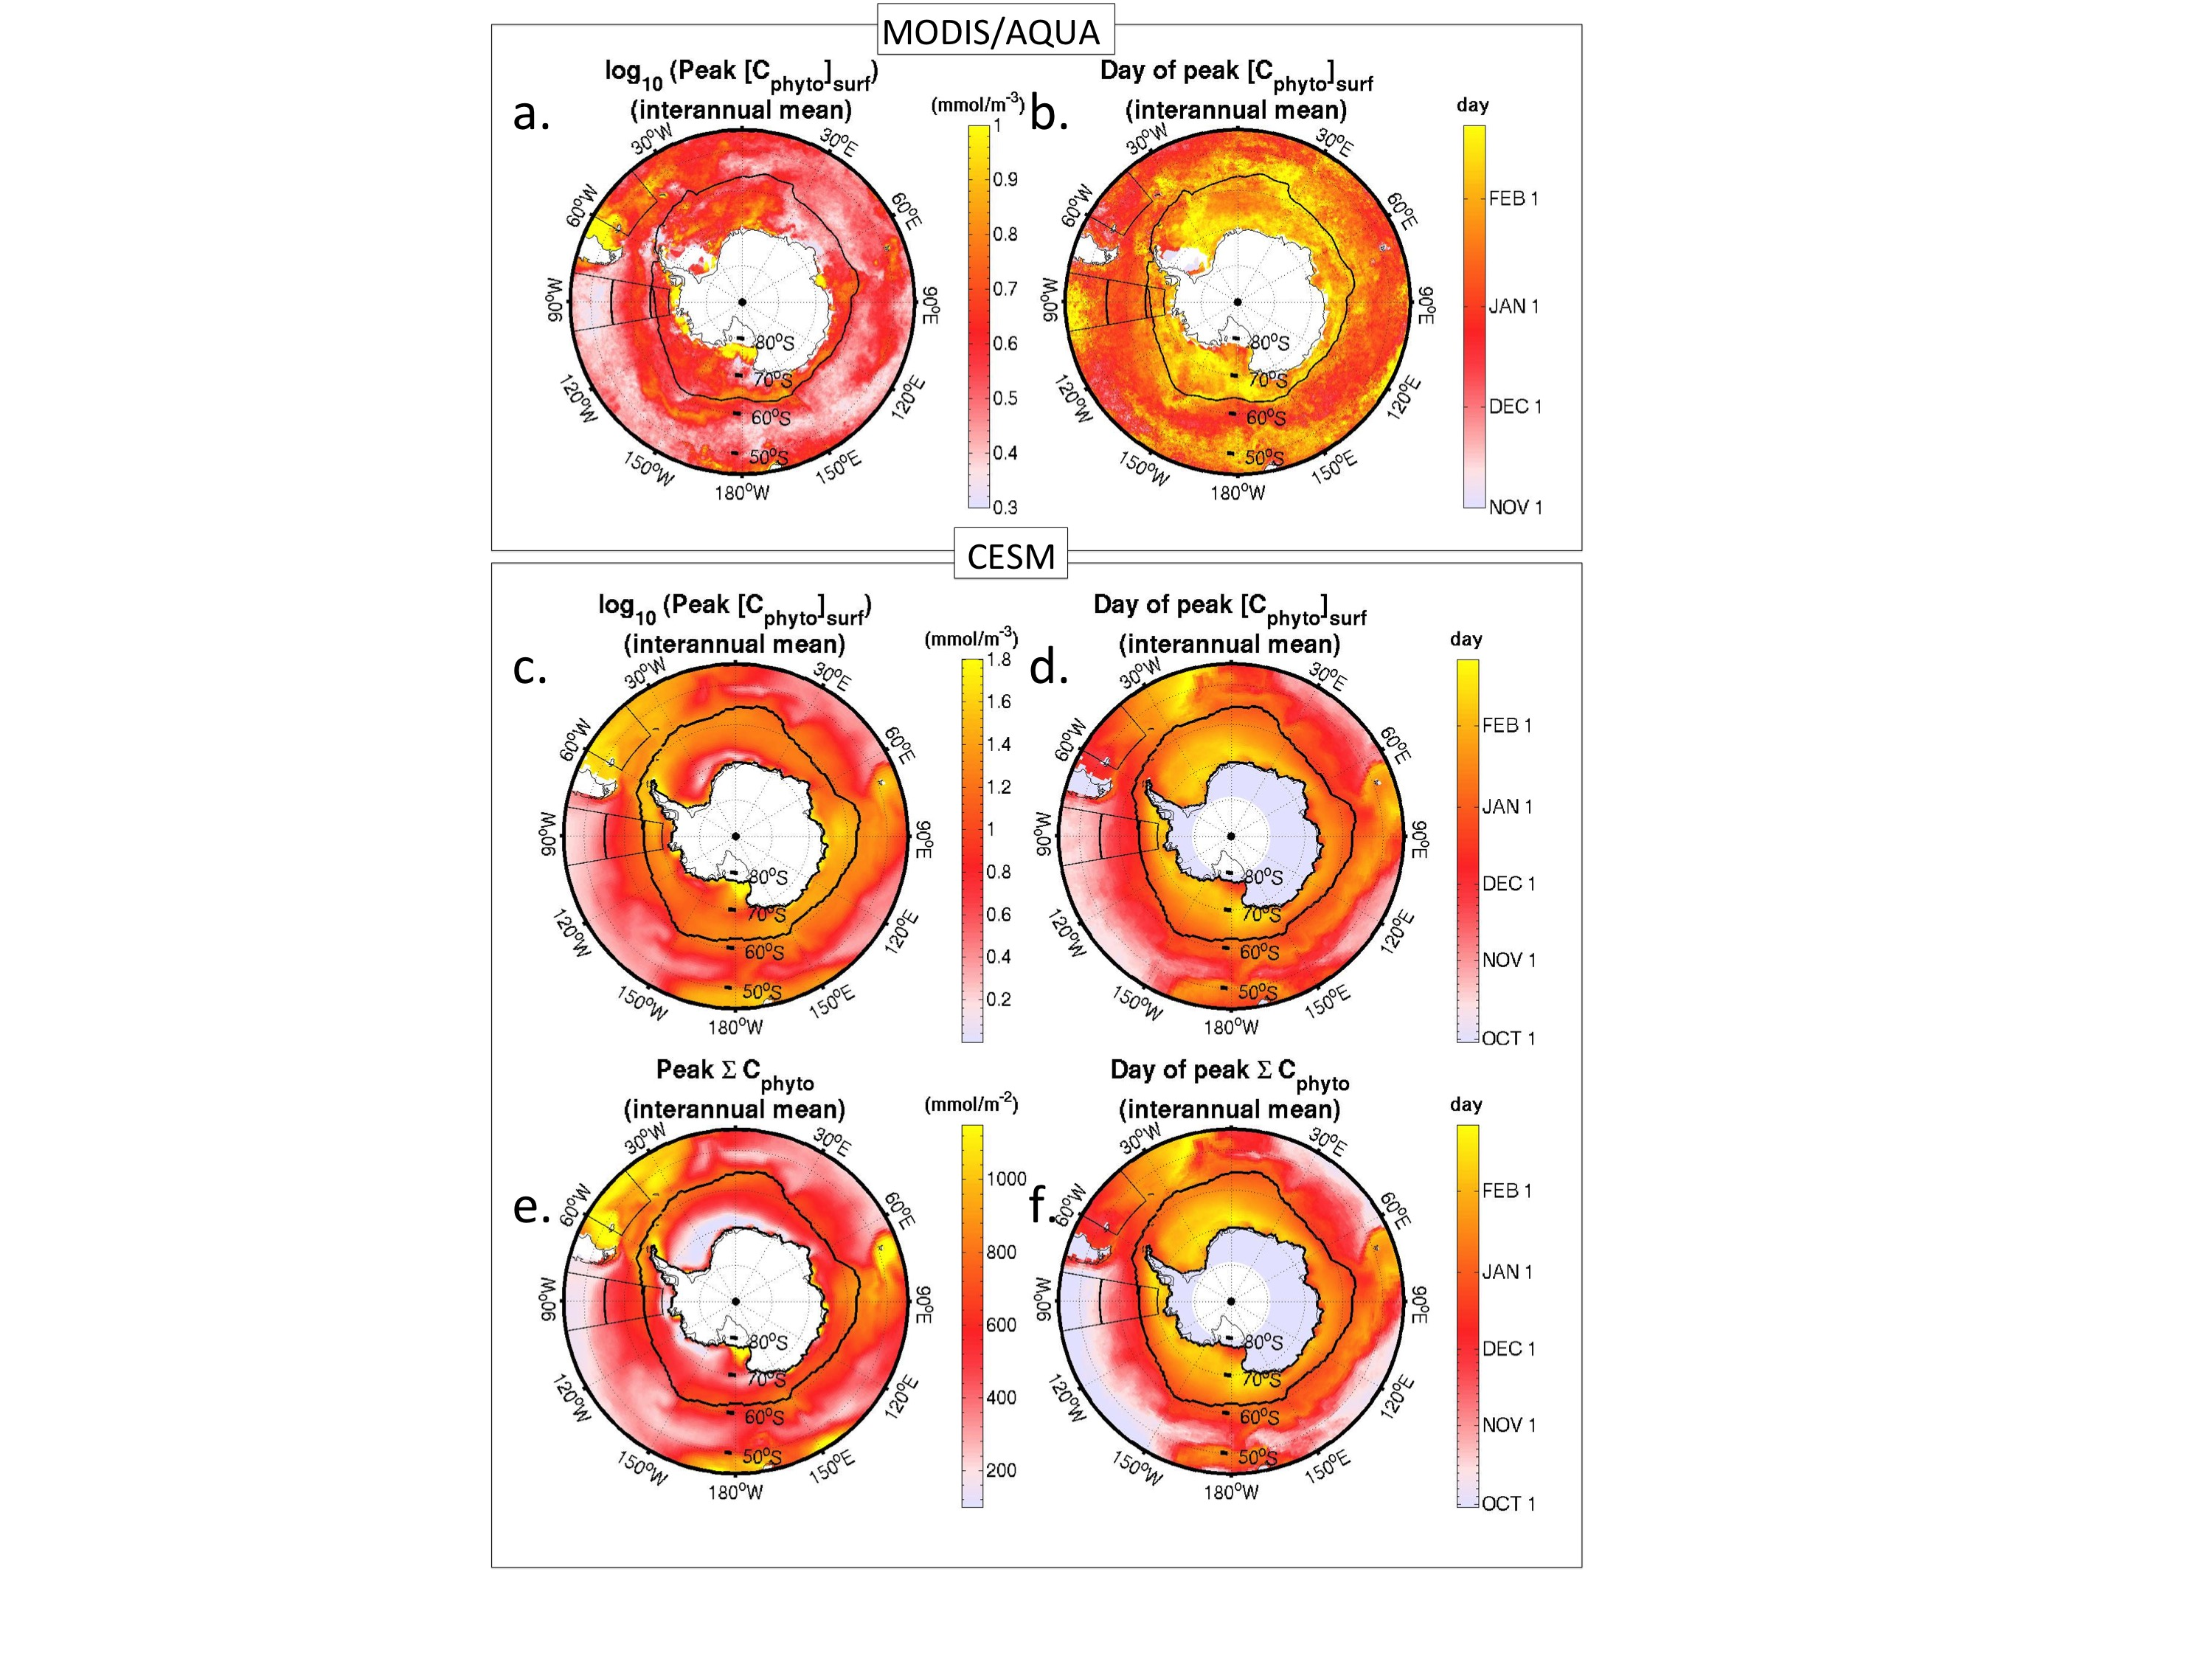
\includegraphics[scale=.2]{figures/Ch2/Figure_1.jpg}
\end{adjustwidth}
\caption[Peak bloom size and timing]{Peak bloom size and timing.  Climatological mean phytoplankton (\textbf{a}) peak surface carbon biomass concentration and (\textbf{b}) day of peak surface carbon biomass concentration plotted from the MODIS/AQUA satellite record. (\textbf{c}) and (\textbf{d}) plot the same metrics from the CESM simulation. Note that subplots (\textbf{a}) and (\textbf{c}) are plotted in $log_{10}$ scale to better capture the spatial distribution. (\textbf{e}) and (\textbf{f}) plot the magnitude and timing of peak carbon biomass inventory as simulated by CESM. In all subplots, the region that sees, on average, at least 15\% mean annual fractional ice coverage is outlined, along with regional bins P1 (55$^\circ$S - 45$^\circ$S, 100$^\circ$W-80$^\circ$W), P2 (65$^\circ$S -55$^\circ$S, 100$^\circ$W-80$^\circ$W), and P3 (70$^\circ$S -65$^\circ$S, 100$^\circ$W-80$^\circ$W) in the Pacific and bin A1 (55$^\circ$S - 45$^\circ$S, 60$^\circ$W-40$^\circ$W) in the Atlantic.}
\label{fig:Fig1}
\end{figure}



%%%%%%%%%%%%%%%%%%%%%%%%
%%%%%% Figure 2 %%%%%%%%
%%%%%%%%%%%%%%%%%%%%%%%%

\begin{figure}[!htbp]
\begin{adjustwidth}{-1in}{-1in}
 \centering
 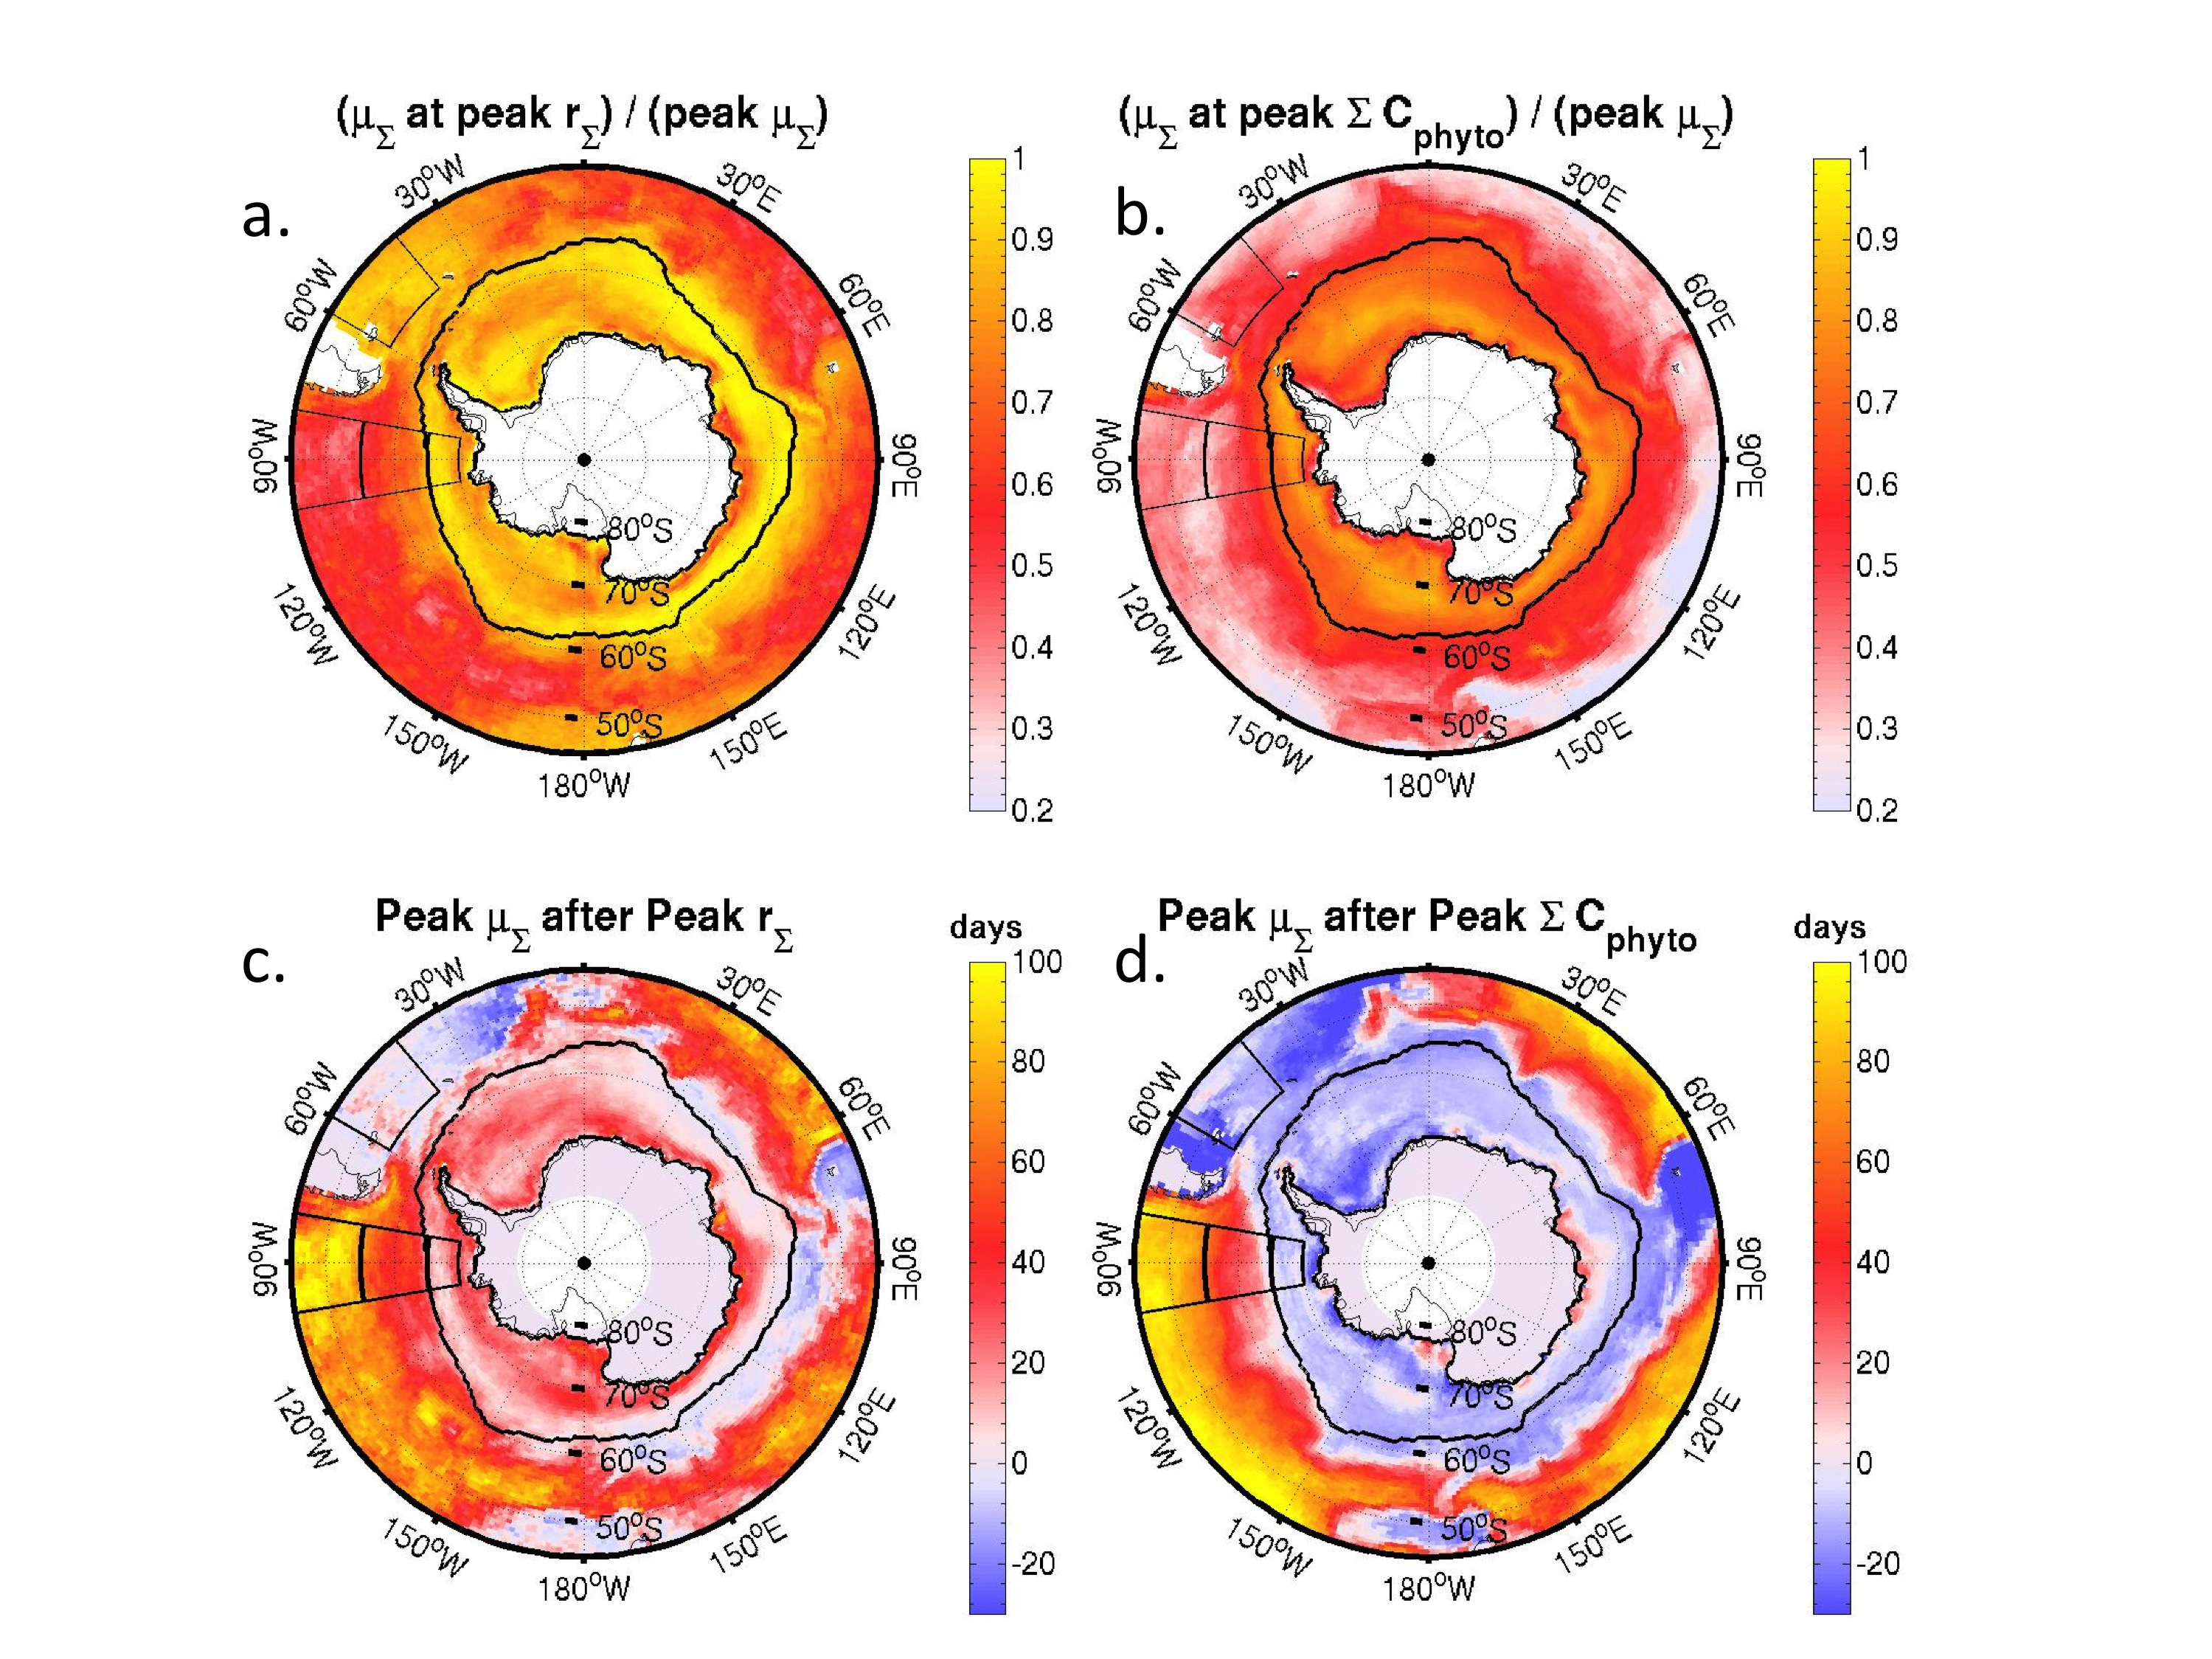
\includegraphics[scale=.2]{figures/Ch2/Figure_2.jpg}
\end{adjustwidth}
\caption[Relative size and timing of simulated depth-integrated phytoplankton specific growth rates]{Relative size and timing of depth-integrated phytoplankton specific growth rates as simulated in CESM. Ratio of population specific division rate ($\mu_\Sigma$) to seasonal peak $\mu_\Sigma$ at time of (\textbf{a}) peak net population specific growth rate $r_\Sigma$ and (\textbf{b}) peak biomass inventory ($\Sigma C_{phyto}$). Number of days $\mu_\Sigma$ occurs after (\textbf{c}) peak $r_\Sigma$ and (\textbf{d}) peak $\Sigma C_{phyto}$. Time series of $\mu_\Sigma$ and  $r_\Sigma$ are first smoothed with a 7-day Hanning window, and metrics are averaged over 30 years of model output.}
\label{fig:Fig2}
\end{figure}


%%%%%%%%%%%%%%%%%%%%%%%%
%%%%%% Figure 3 %%%%%%%%
%%%%%%%%%%%%%%%%%%%%%%%%

\begin{figure}[!htbp]
\begin{adjustwidth}{-1in}{-1in}
 \centering
 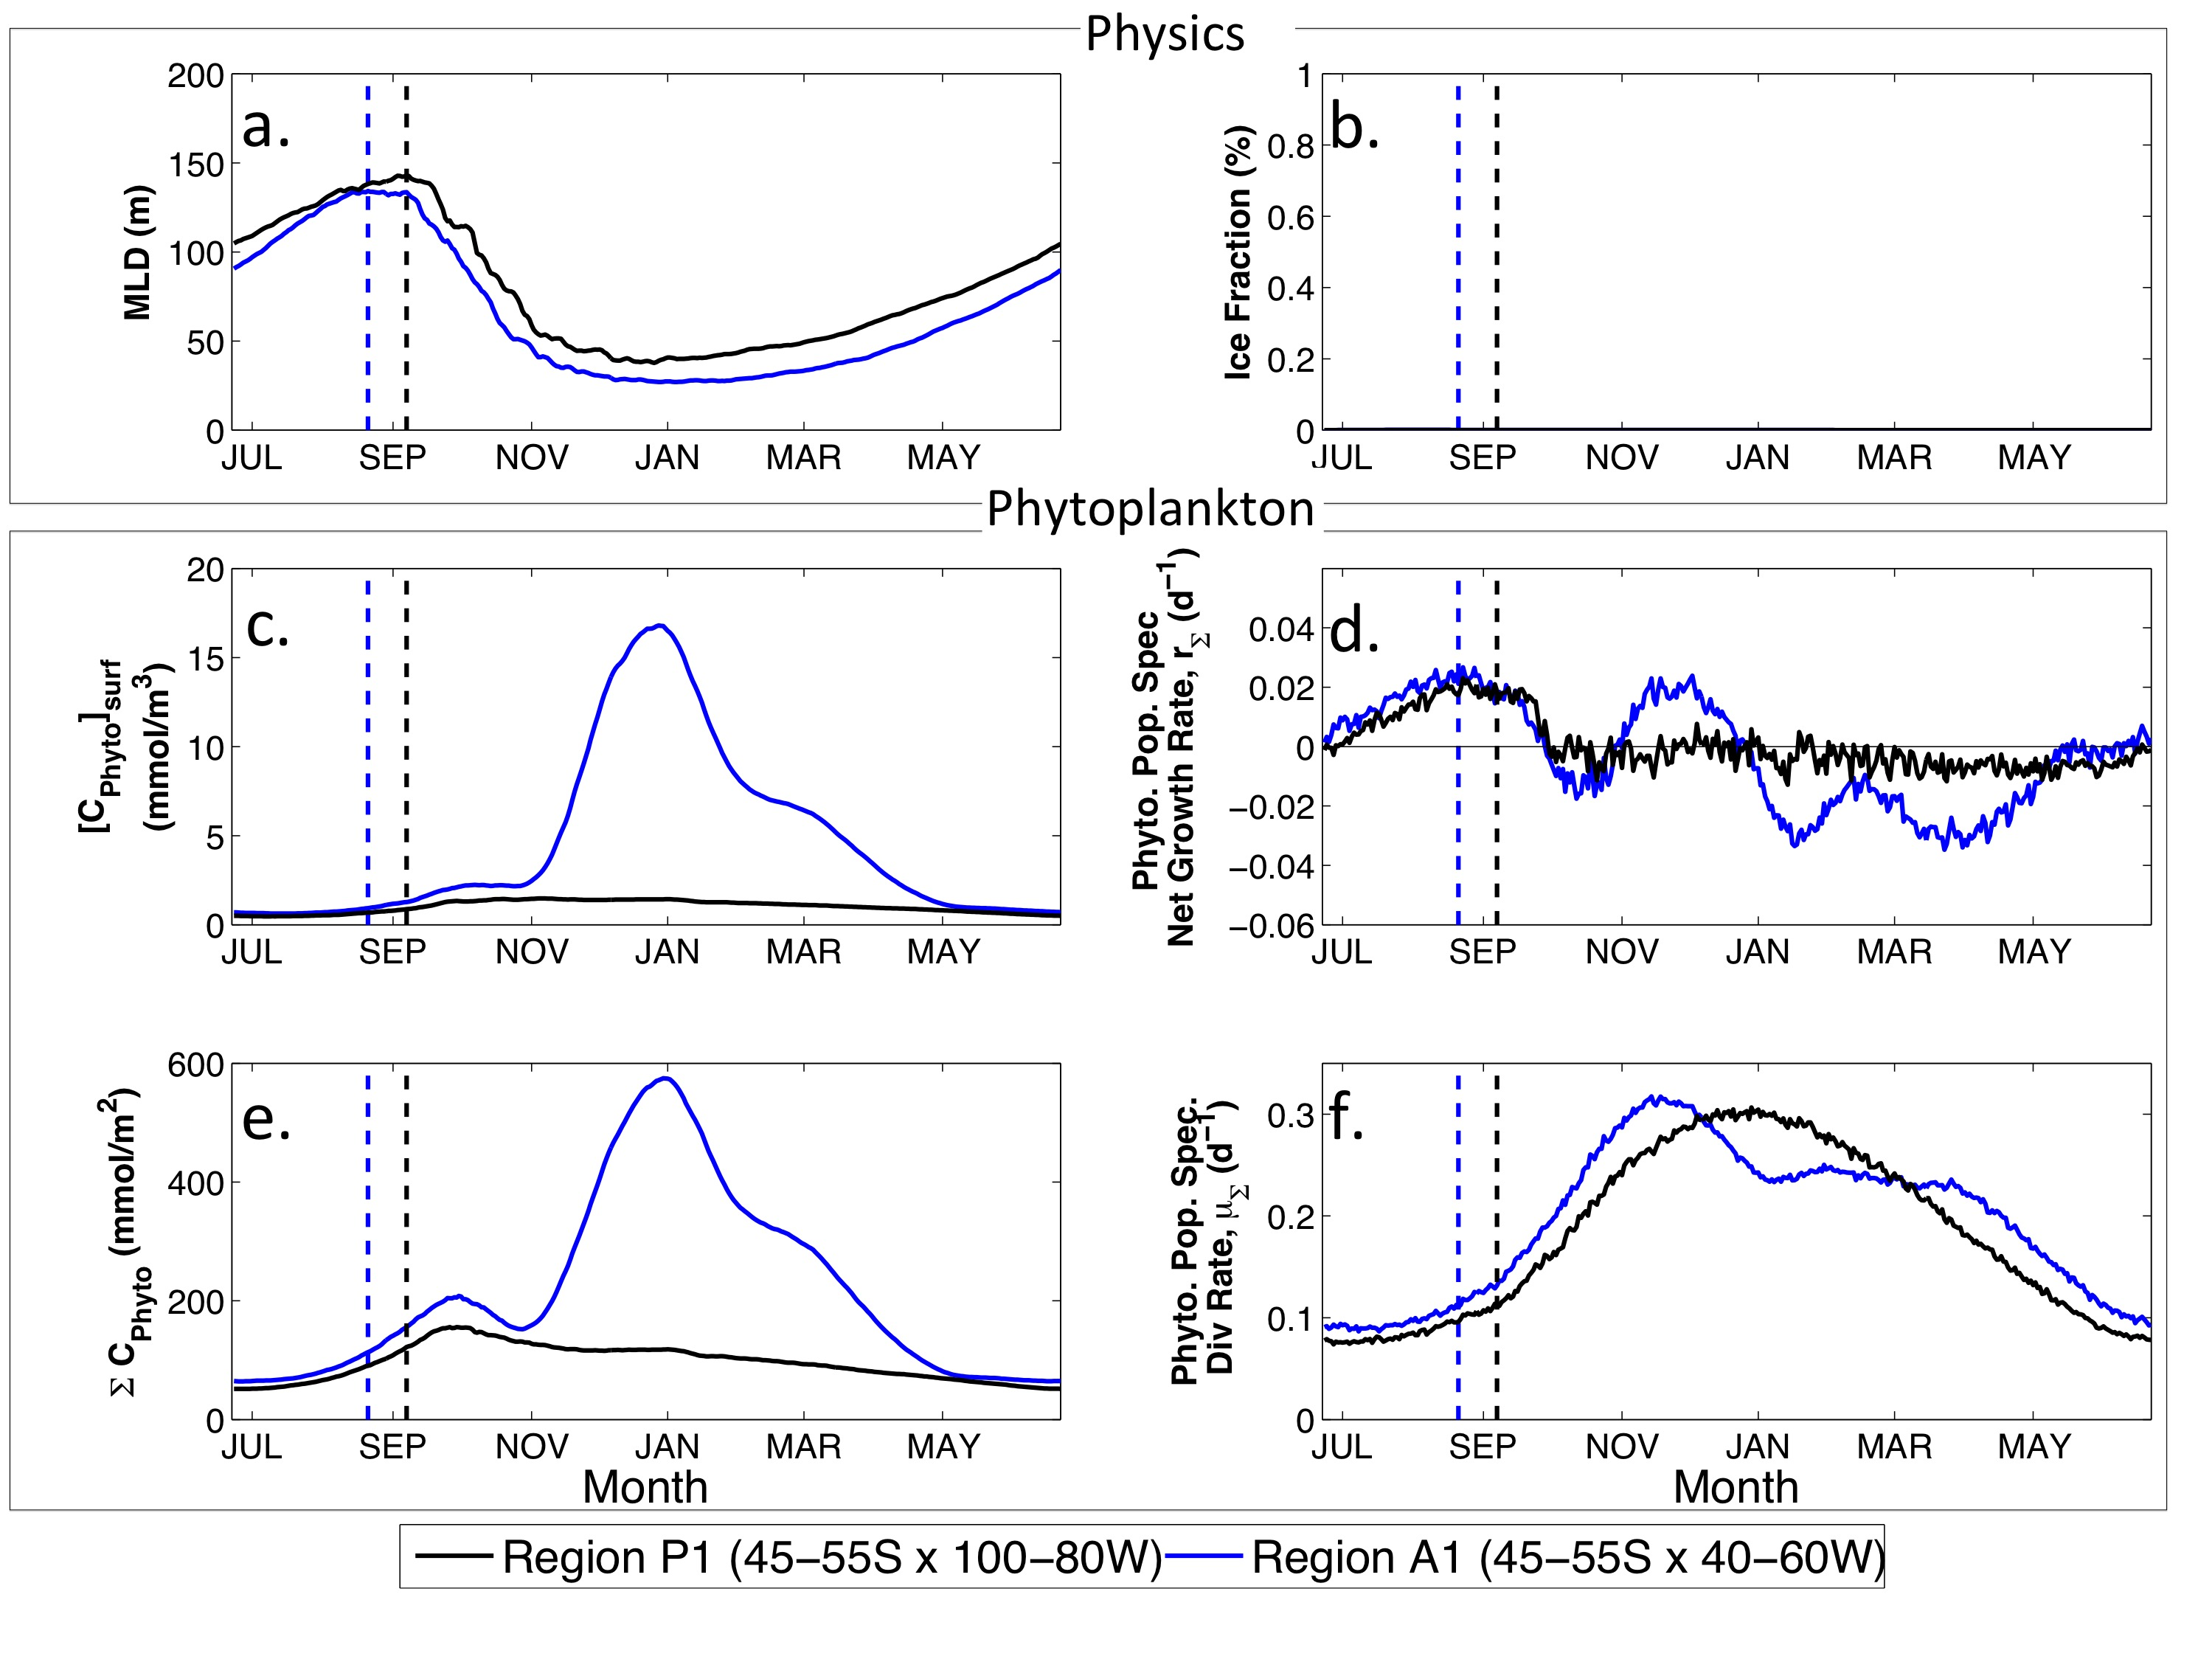
\includegraphics[scale=.18]{figures/Ch2/Figure_3.jpg}
\end{adjustwidth}
\caption[Regionally averaged, seasonal climatologies simulated by CESM; A1 and P1]{Regionally averaged, seasonal climatologies simulated by CESM for A1 and P1. (\textbf{a}) $MLD$ (\textbf{b}) ice fraction (not applicable) (\textbf{c}) $[C_{phyto}]_{surf}$  (\textbf{d}) $r_\Sigma$ (\textbf{e}) $\Sigma C_{phyto}$ (\textbf{f}) $\mu_\Sigma$. The SE Pacific bin (P1: 55$^\circ$S -45$^\circ$S, 100$^\circ$W-80$^\circ$W) is plotted in black, and the SW Atlantic Bin (A1: 55$^\circ$S -45$^\circ$S, 60$^\circ$W-40$^\circ$W) in blue. The timing of the climatological maximum mixed layer depth is marked by a dashed line of the according color.}
\label{fig:Fig3}
\end{figure}


%%%%%%%%%%%%%%%%%%%%%%%%
%%%%%% Figure 4 %%%%%%%%
%%%%%%%%%%%%%%%%%%%%%%%%

\begin{figure}[!htbp]
\begin{adjustwidth}{-1in}{-1in}
 \centering
 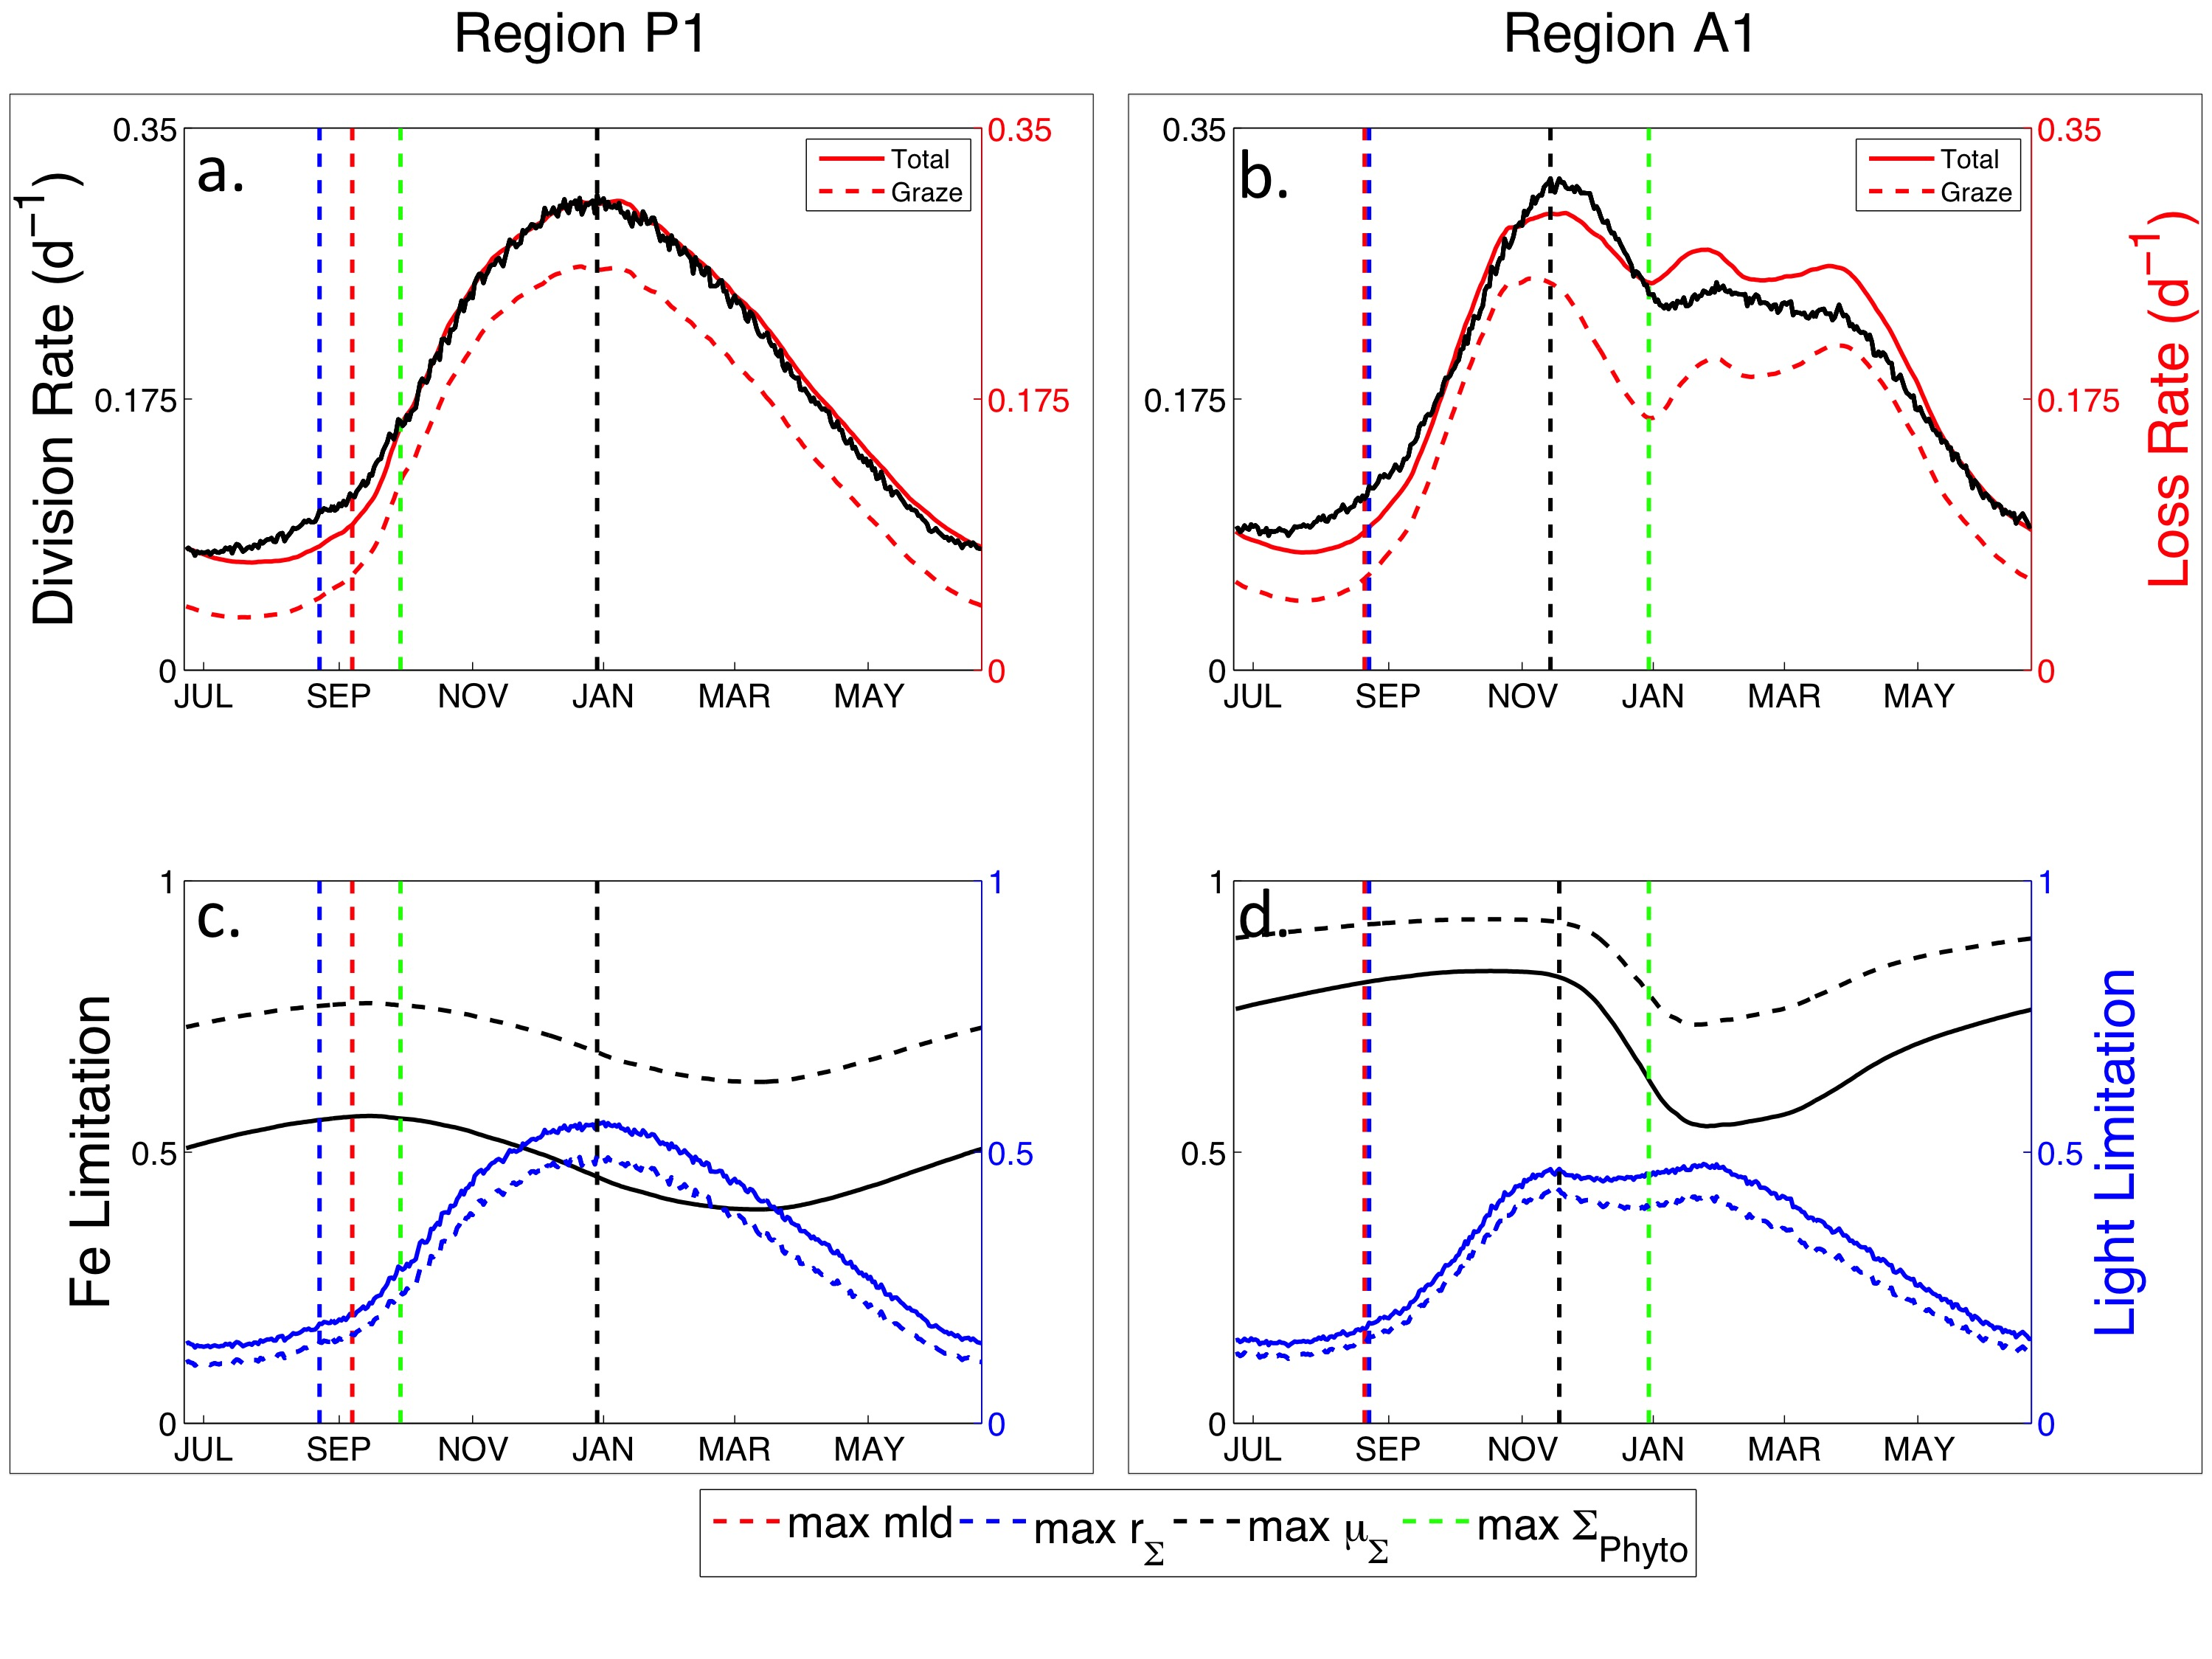
\includegraphics[scale=.18]{figures/Ch2/Figure_4.jpg}
\end{adjustwidth}
\caption[Simulated seasonal climatologies of phytoplankton rate and limitation terms; Bin P1 and A1]{Seasonal climatologies of phytoplankton rate (\textbf{a, b}) and limitation (\textbf{c, d}) terms simulated by CESM averaged over Bin P1 (\textbf{a, c}) and A1 (\textbf{b, d}). (\textbf{a, b}) Population specific cell division rate (black), total loss rate (red solid), and grazing rate (red dashed). (\textbf{c, d}) Limitation terms averaged over the profile depth ($Z_{profile}$) for iron (black; consistently the most limiting nutrient) and light (blue) with diatom (solid) and small phytoplankton (dashed). Vertical dashed lines refer to the climatologic timing of the maximum $MLD$ (red), population specific net growth rates (blue), population specific division rates (black) and phytoplankton biomass inventory (green).
}
\label{fig:Fig4}
\end{figure}

%%%%%%%%%%%%%%%%%%%%%%%%
%%%%%% Figure 5 %%%%%%%%
%%%%%%%%%%%%%%%%%%%%%%%%

\begin{figure}[!htbp]
\begin{adjustwidth}{-1in}{-1in}
 \centering
 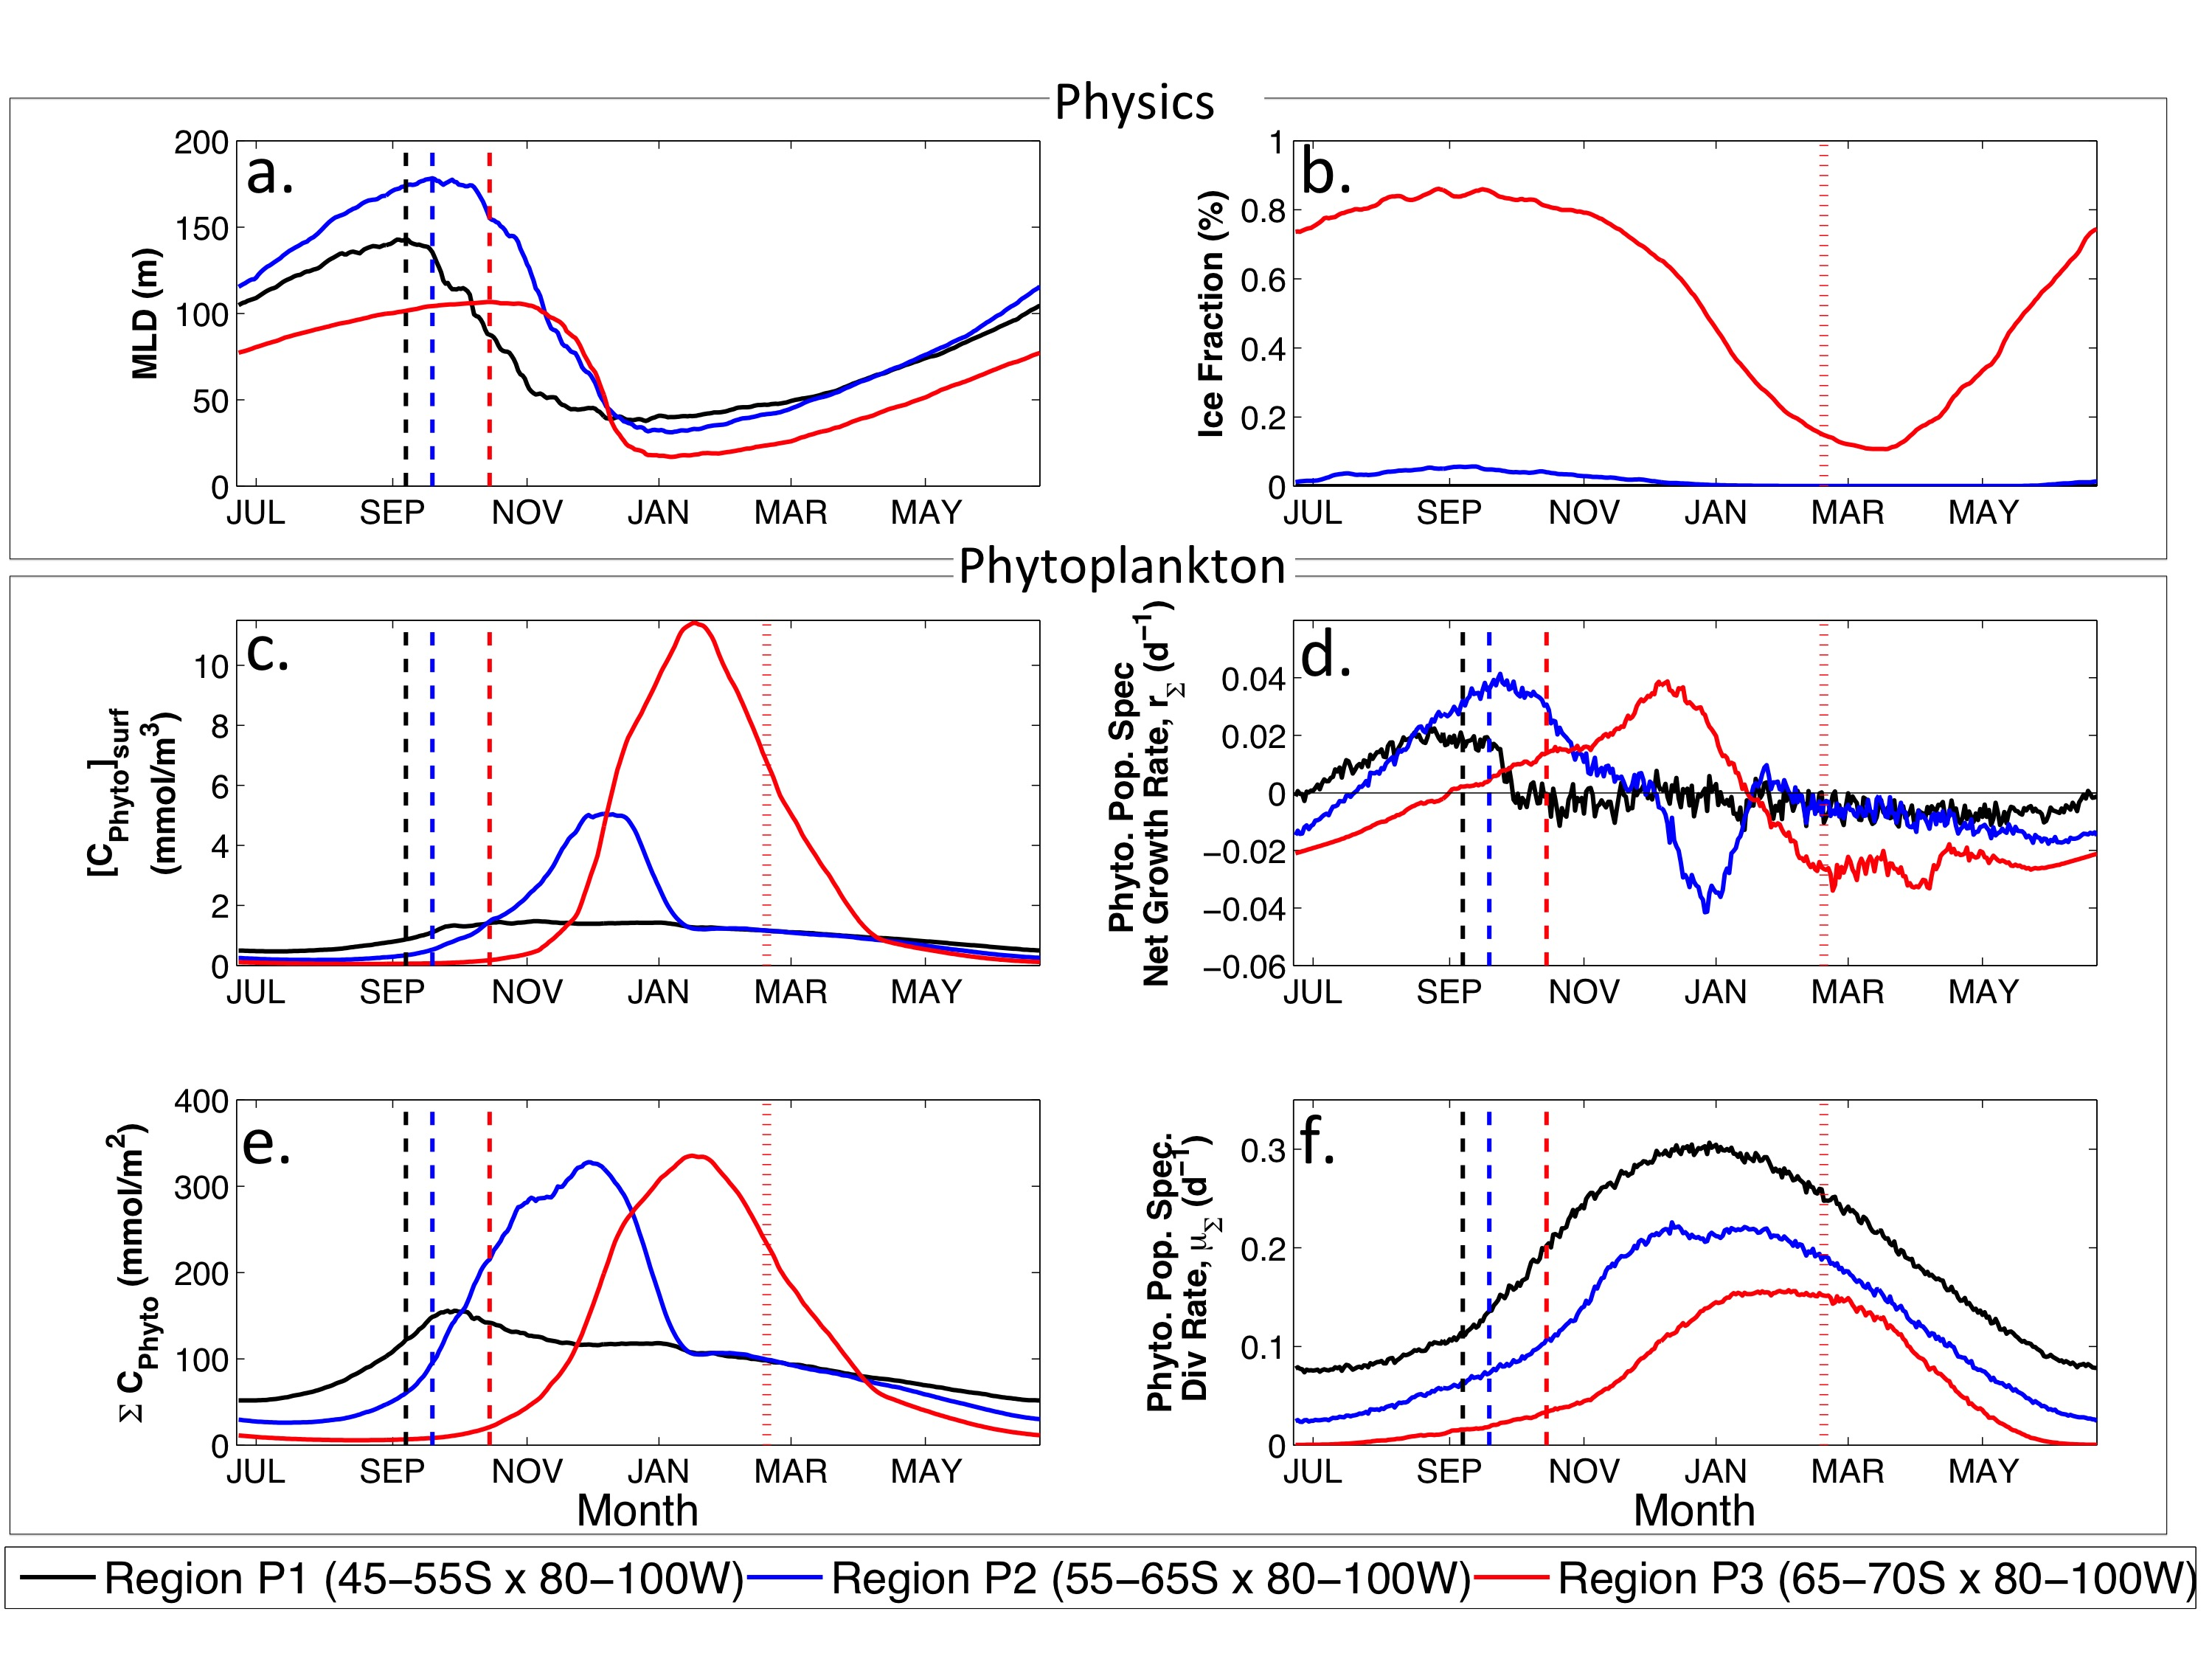
\includegraphics[scale=.18]{figures/Ch2/Figure_5.jpg}
\end{adjustwidth}
\caption[Regionally averaged, seasonal climatologies simulated by CESM; P1, P2, and P3]{Regionally averaged, seasonal climatologies simulated by CESM for P1, P2, and P3. (\textbf{a}) $MLD$ (\textbf{b}) ice fraction (not applicable) (\textbf{c}) $[C_{phyto}]_{surf}$  (\textbf{d}) $r_\Sigma$ (\textbf{e}) $\Sigma C_{phyto}$ (\textbf{f}) $\mu_\Sigma$. The lowest latitude bin (P1: 55$^\circ$S -45$^\circ$S, 100$^\circ$W-80$^\circ$W) is plotted in black, the ‘middle’ latitude bin (P2: 65$^\circ$S -55$^\circ$S, 100$^\circ$W-80$^\circ$W) in blue and the highest latitude bin (70$^\circ$S - 65$^\circ$S, 100$^\circ$W-80$^\circ$W) in black. The timing of the climatological maximum mixed layer depth is marked by a dashed line of the according color, and a color coated dotted line marks the climatologic timing of sea ice retreat where applicable (here only in Region P3). 
}
\label{fig:Fig5}
\end{figure}



%%%%%%%%%%%%%%%%%%%%%%%%
%%%%%% Figure 6 %%%%%%%%
%%%%%%%%%%%%%%%%%%%%%%%%

\begin{figure}[!htbp]
\begin{adjustwidth}{-1in}{-1in}
 \centering
 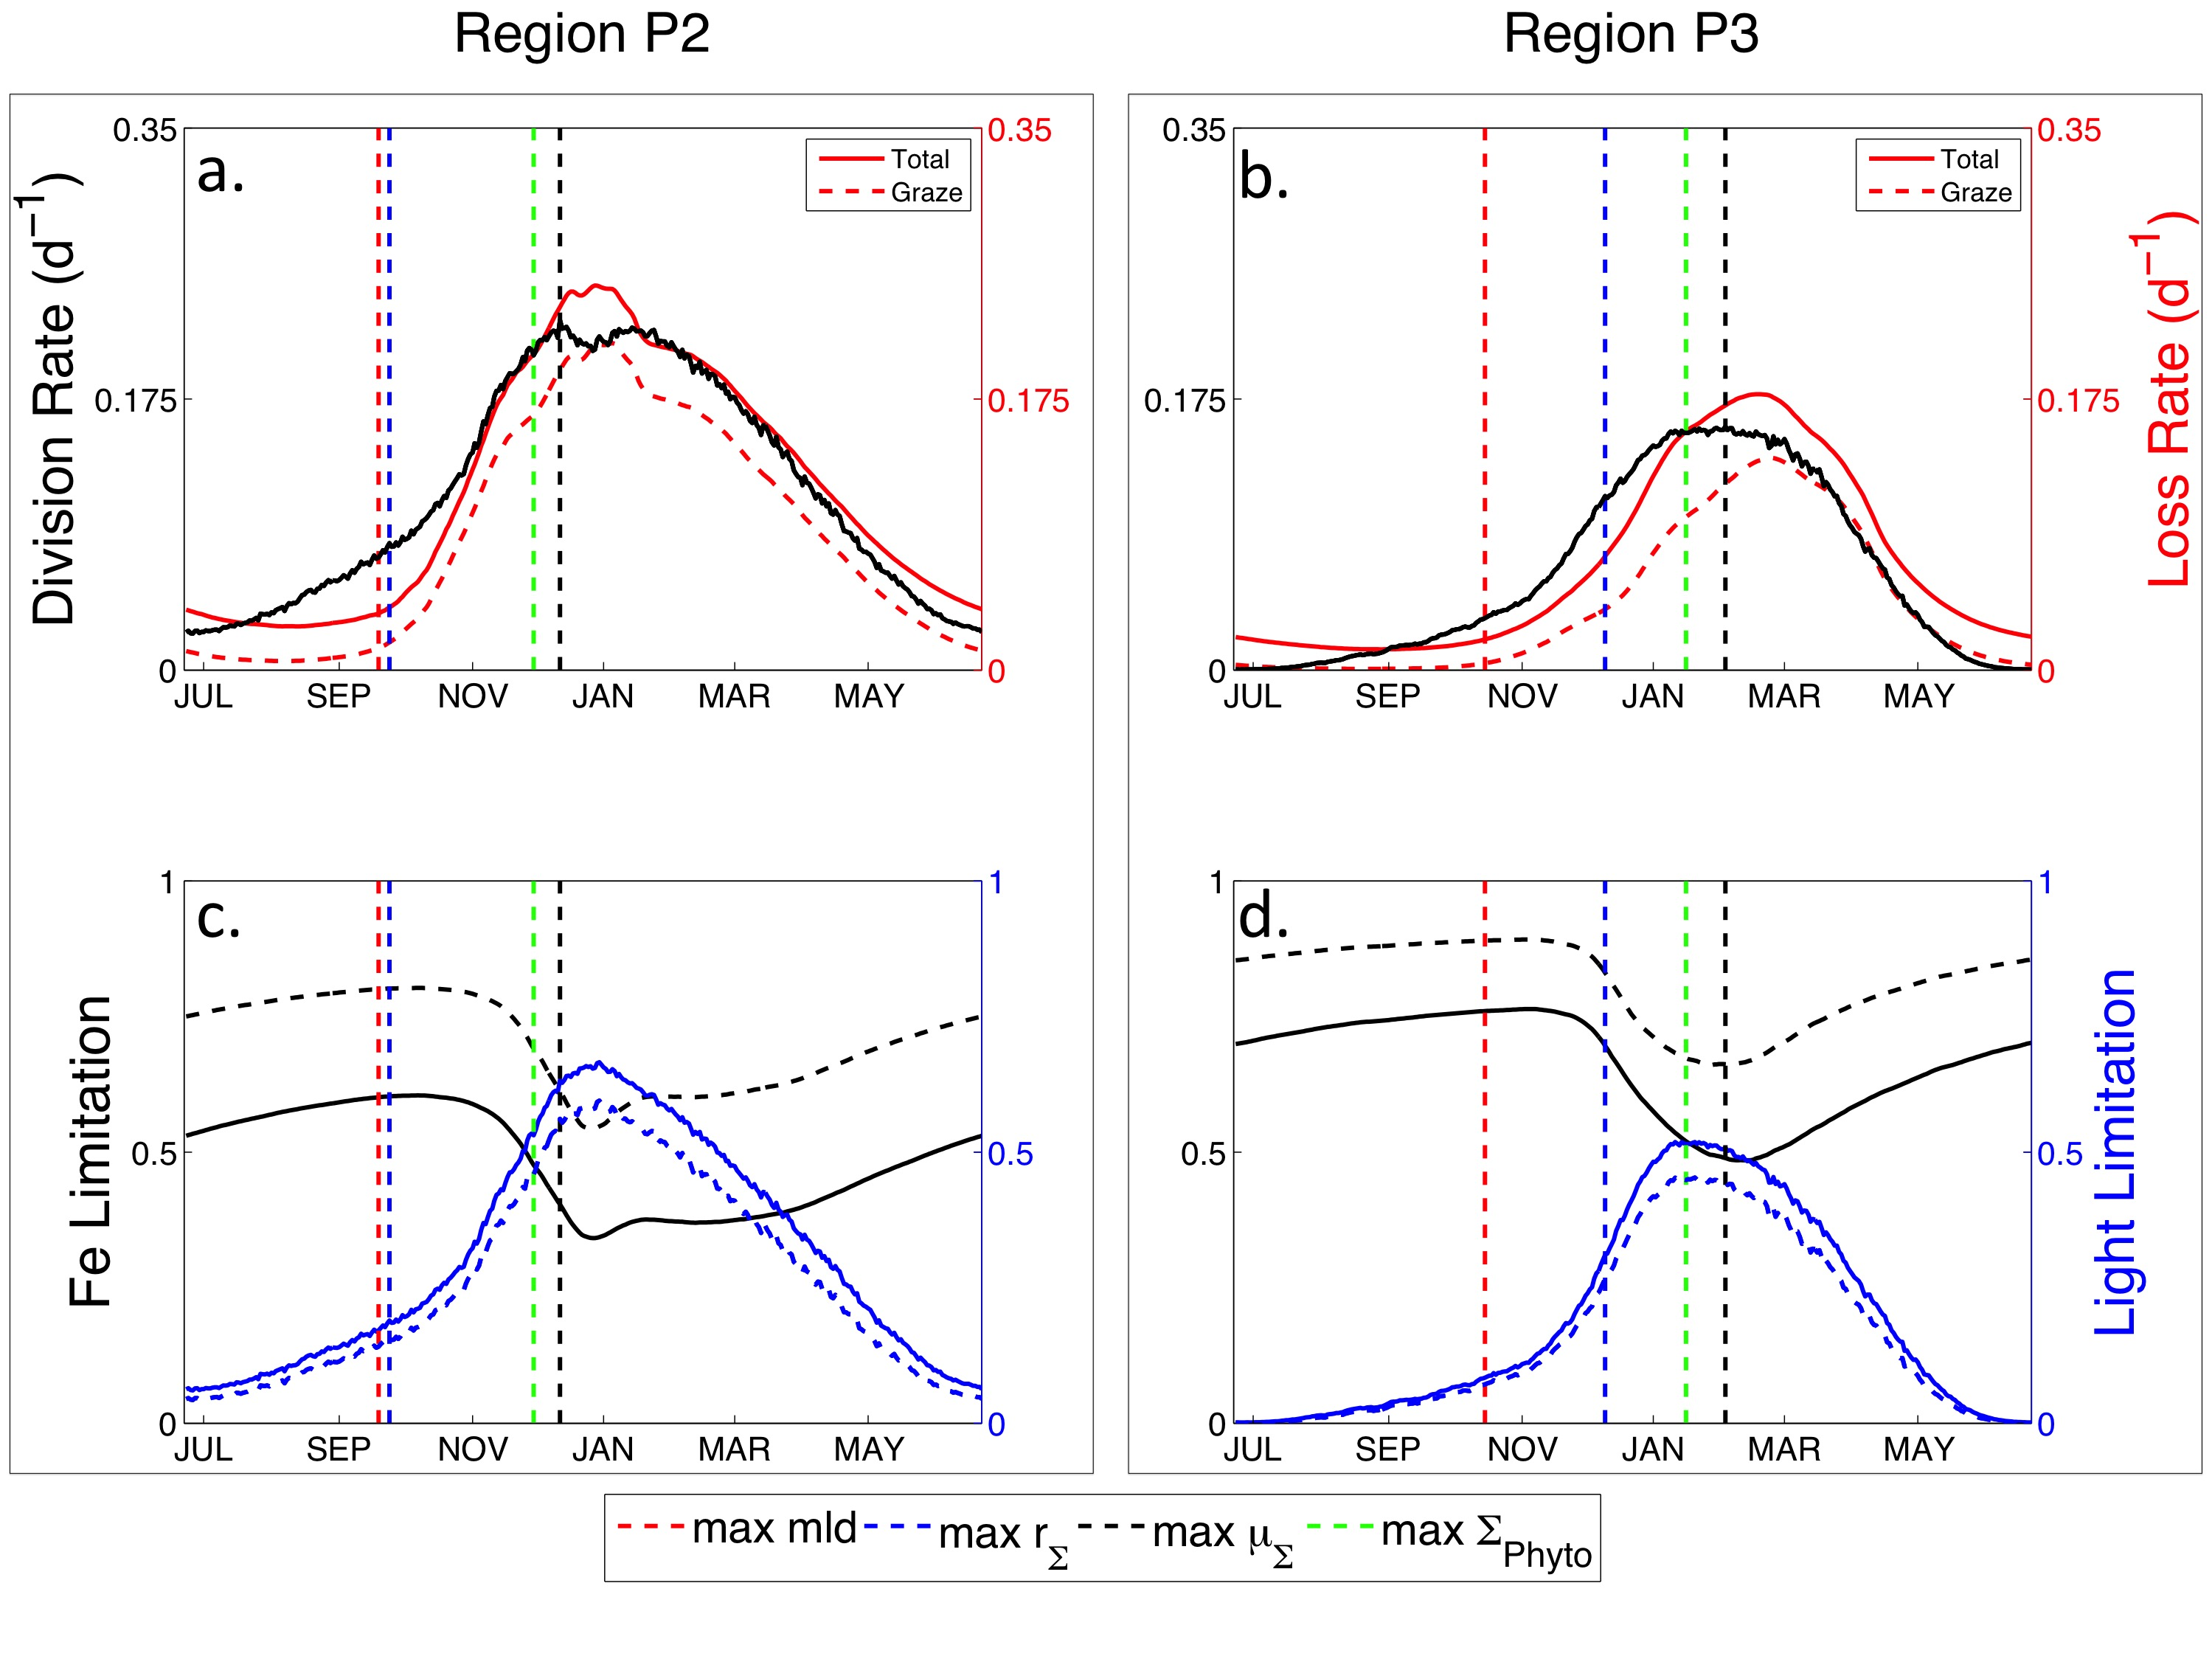
\includegraphics[scale=.18]{figures/Ch2/Figure_6.jpg}
\end{adjustwidth}
\caption[Simulated seasonal climatologies of phytoplankton rate and limitation terms; Bin P1, P2, and P3]{Seasonal climatologies of phytoplankton rate (\textbf{a, b}) and limitation (\textbf{c, d}) terms simulated by CESM averaged over Bin P1 (\textbf{a, c}) and A1 (\textbf{b, d}). (\textbf{a, b}) Population specific cell division rate (black), total loss rate (red solid), and grazing rate (red dashed). (\textbf{c, d}) Limitation terms averaged over the profile depth ($Z_{profile}$) for iron (black; consistently the most limiting nutrient) and light (blue) with diatom (solid) and small phytoplankton (dashed). Vertical dashed lines refer to the climatologic timing of the maximum $MLD$ (red), population specific net growth rates (blue), population specific division rates (black) and phytoplankton biomass inventory (green).}
\label{fig:Fig6}
\end{figure}

%%%%%%%%%%%%%%%%%%%%%%%%
%%%%%% Figure 7 %%%%%%%%
%%%%%%%%%%%%%%%%%%%%%%%%

\begin{figure}[!htbp]
\begin{adjustwidth}{-1in}{-1in}
 \centering
 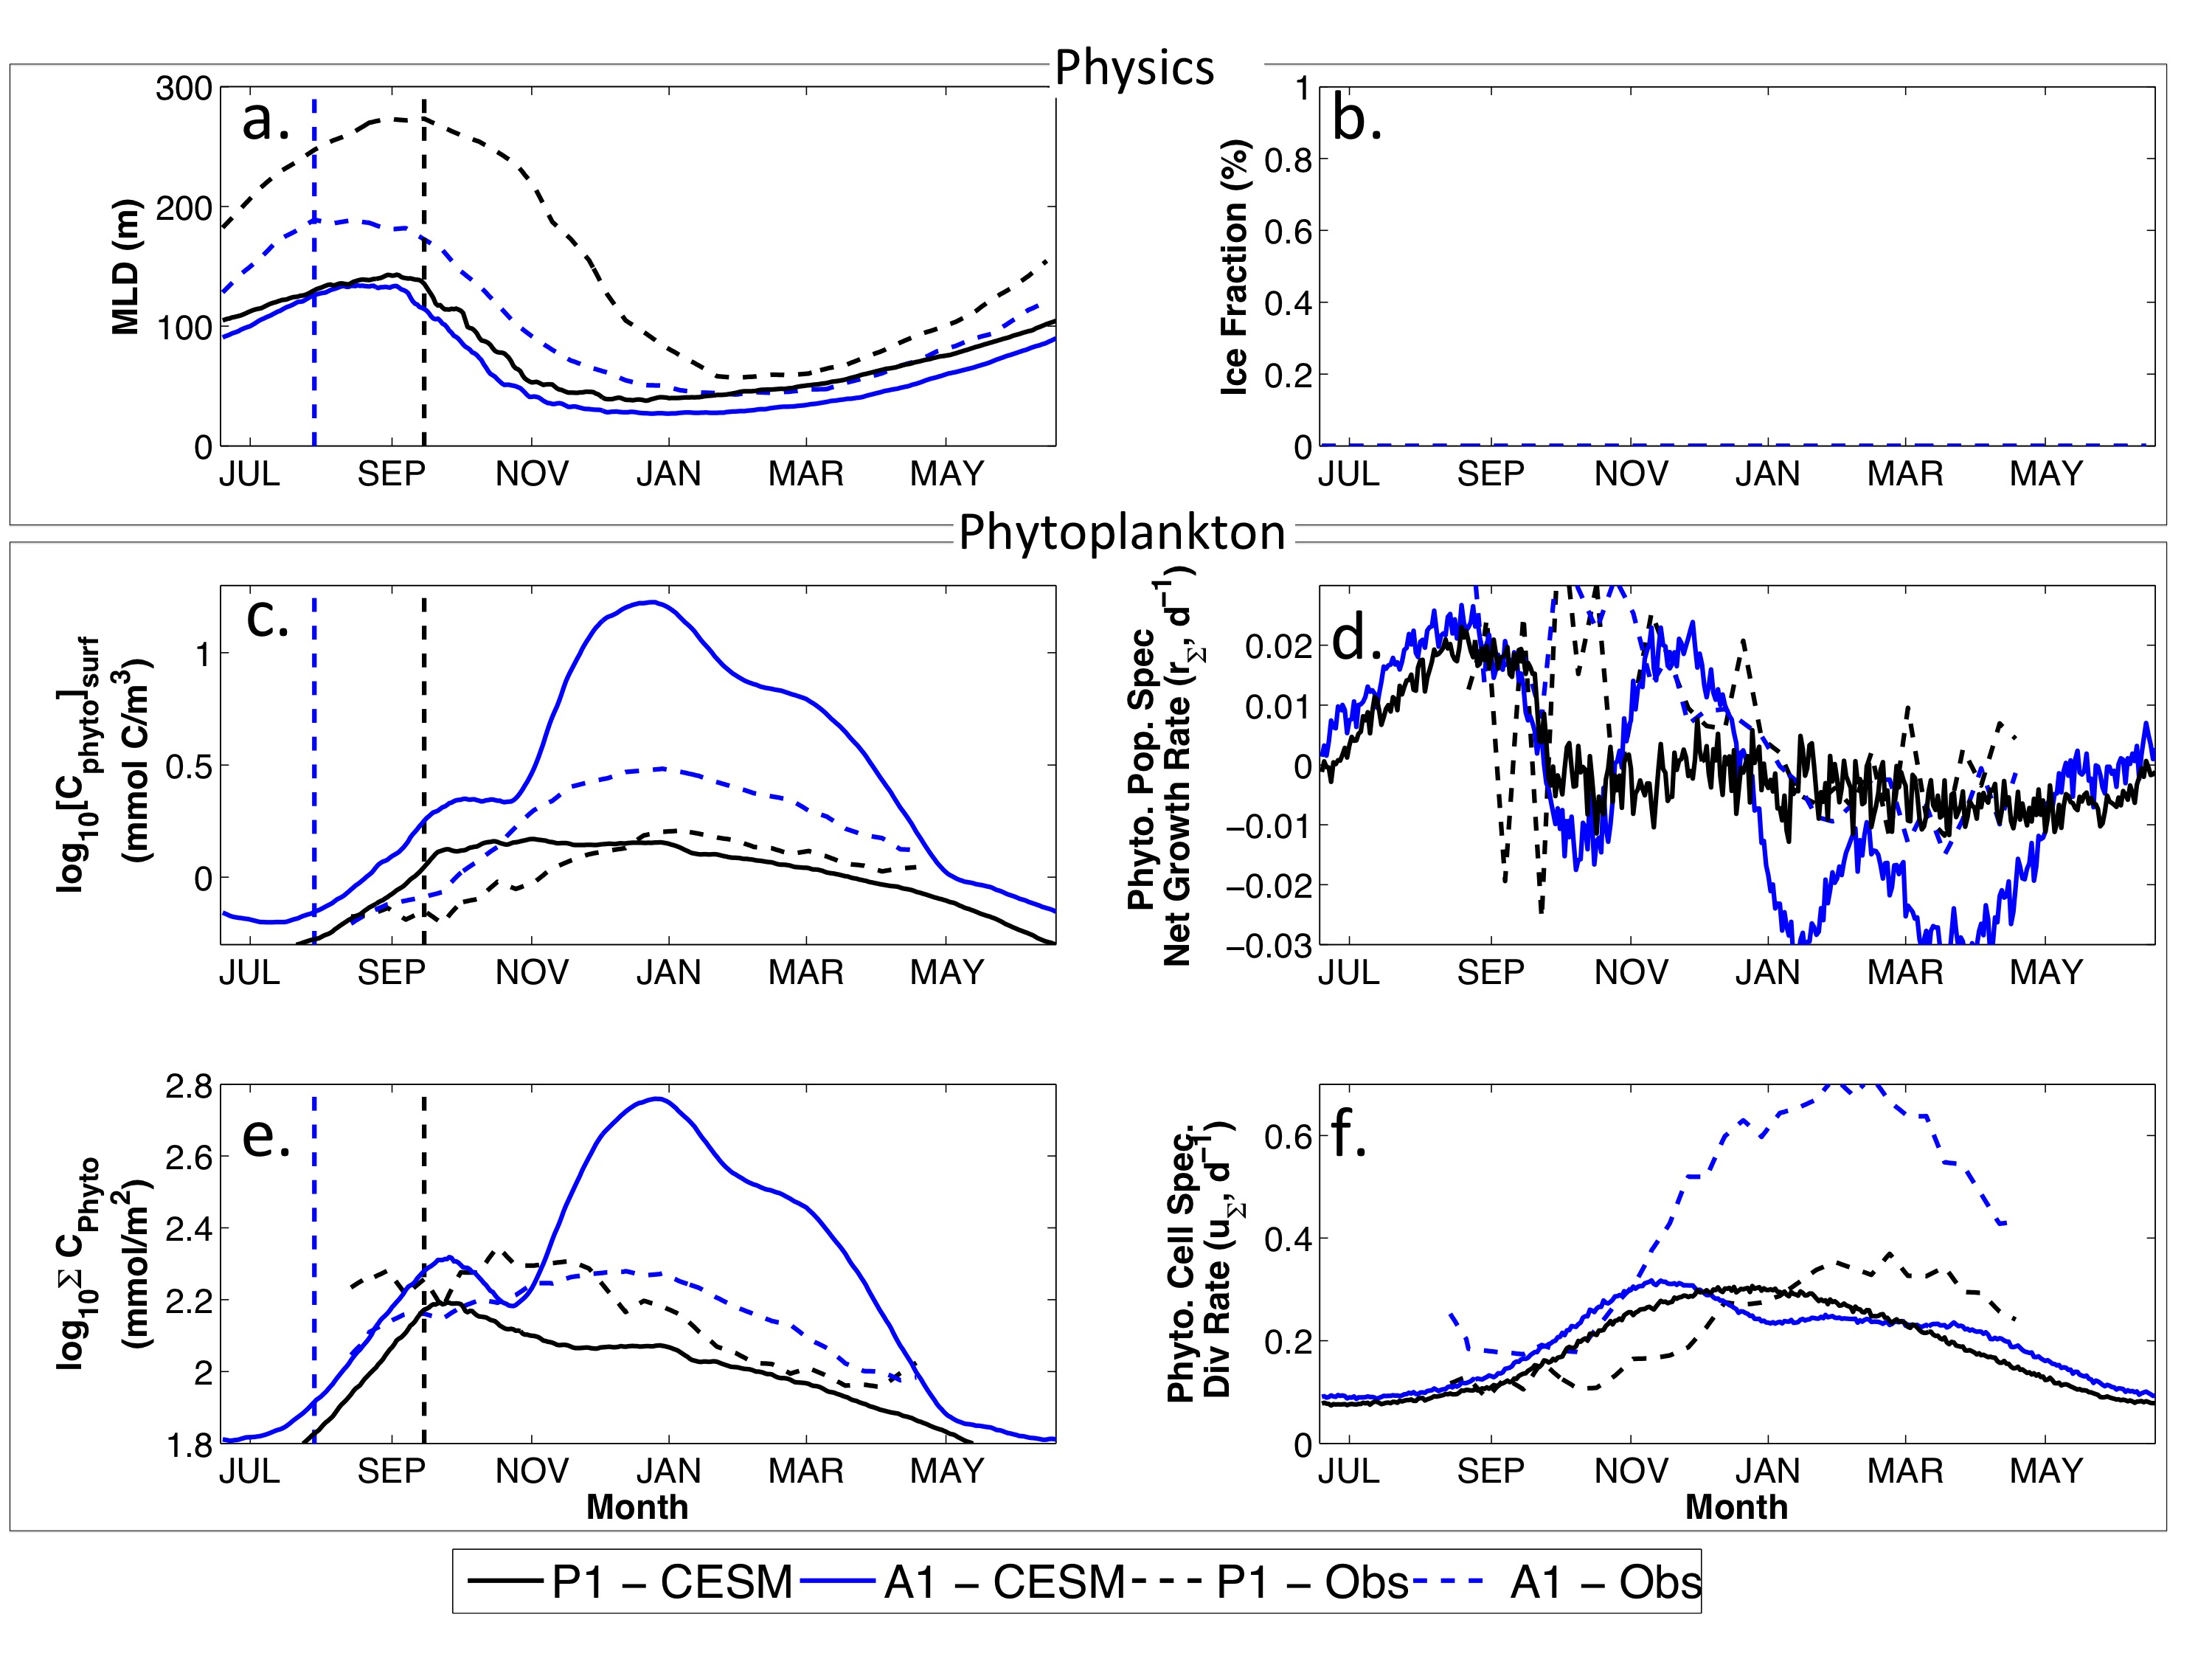
\includegraphics[scale=.18]{figures/Ch2/Figure_7.jpg}
\end{adjustwidth}
\caption[Observational and simulated regional climatologies; Bins P1 and A1]{Observational and simulated regional climatologies for P1 (Black) and A1(Blue) (\textbf{a}) HYCOM/FNMOC reanalyzed (dashed) and simulated (solid) MLD, MODIS observed (dashed) and simulated (solid) phytoplankton (\textbf{c}) biomass concentrations, (\textbf{d}) population specific net growth rates, (\textbf{e}) inventories, (\textbf{f}) and population specific division rates. A dashed line of the according color marks the timing of the climatologic HYCOM/FNMOC reanalyzed maximum mixed layer depth in \textbf{a, c} and \textbf{e}. Simulated traces are identical to \textbf{Fig. 3}, however concentration and inventory are now plotted on log scale.}
\label{fig:Fig7}
\end{figure}


%%%%%%%%%%%%%%%%%%%%%%%%
%%%%%% Figure 8 %%%%%%%%
%%%%%%%%%%%%%%%%%%%%%%%%

\begin{figure}[!htbp]
\begin{adjustwidth}{-1in}{-1in}
 \centering
 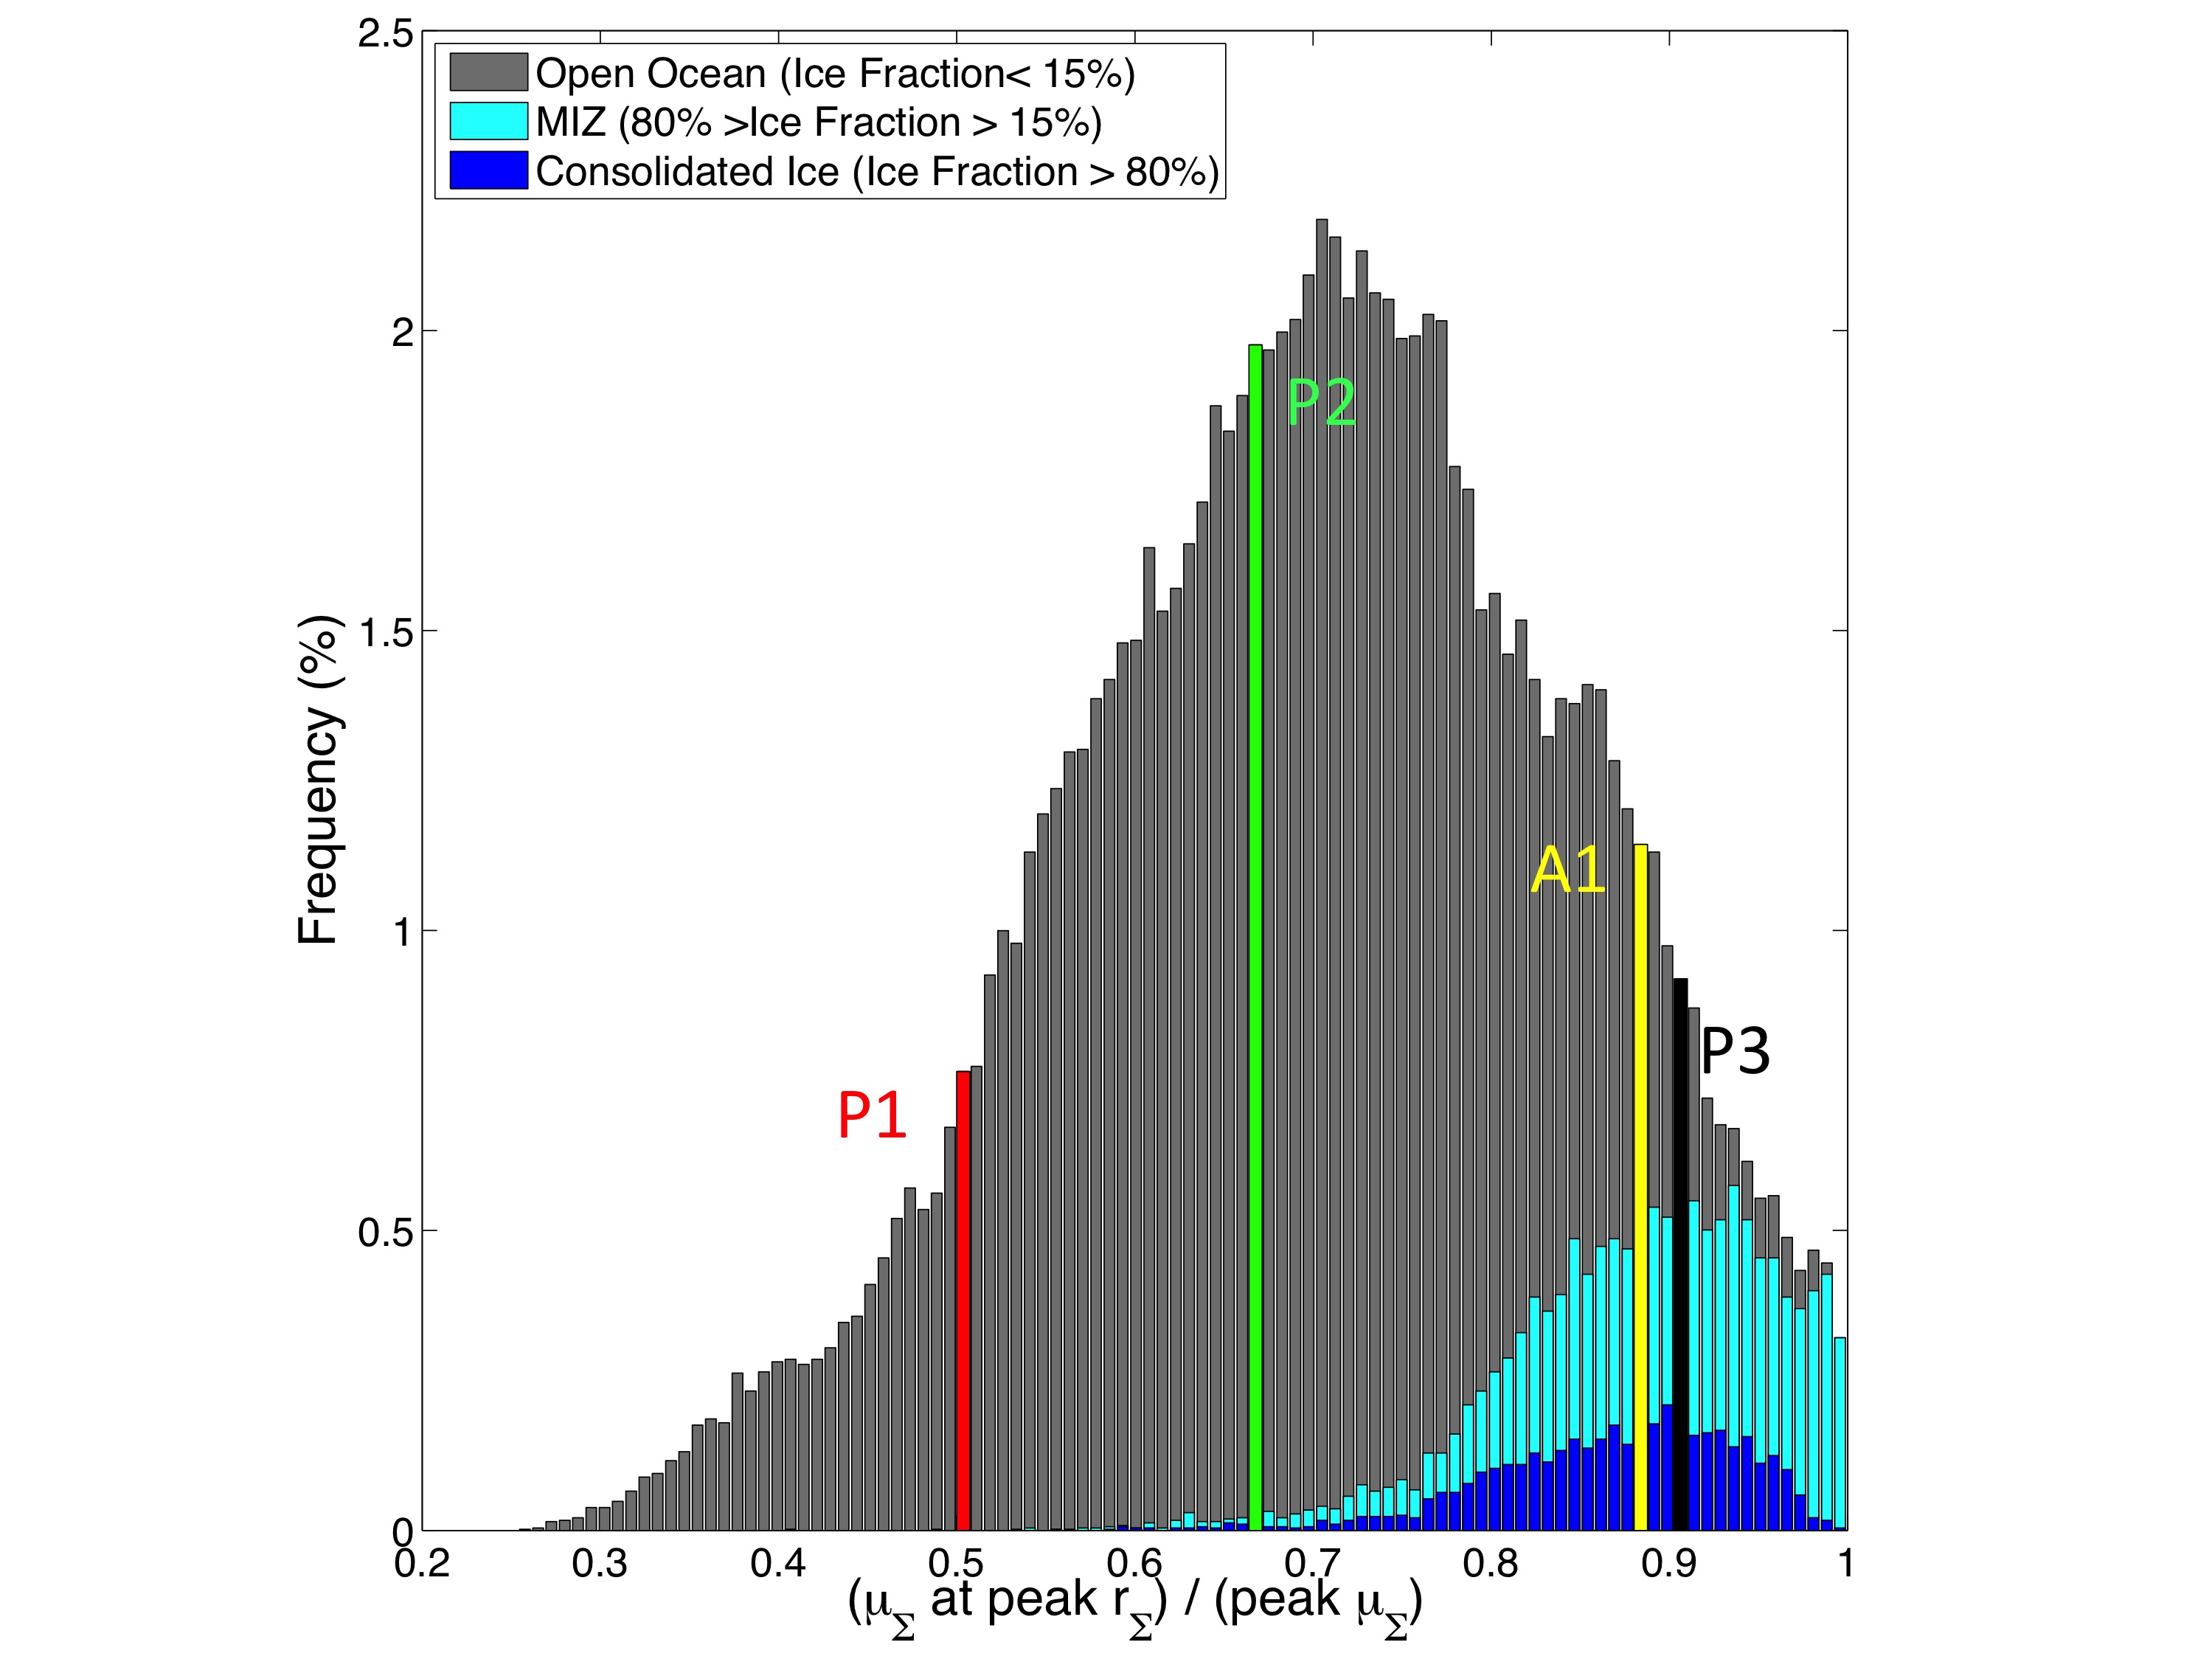
\includegraphics[scale=.2]{figures/Ch2/Figure_8.jpg}
\end{adjustwidth}
\caption[The frequency distribution of $\frac{\mu_\Sigma \textrm{at peak} r_\Sigma}{\textrm{peak} \mu_\Sigma}$]{The frequency distribution of $\frac{\mu_\Sigma \textrm{at peak} r_\Sigma}{\textrm{peak} \mu_\Sigma}$ for all 47,314 Southern Ocean grid cells plotted in \textbf{Fig. 2a}. The corresponding bins for the regional mean $\frac{\mu_\Sigma \textrm{at peak} r_\Sigma}{\textrm{peak} \mu_\Sigma}$ of grid cells in P1 (red), P2 (green), P3 (black), and A1 (yellow) is delineated and color-coded for reference. Each bin is decomposed into the fraction of grid cells within the consolidated ice zone (blue), the $MIZ$ (cyan), and open-ocean (grey). Following \parencite{StroeveMappingassessingvariability2016}, the $MIZ$ is defined as a mean annual ice fraction between 15\% and 80\%, the consolidated ice zone as a mean annual fraction above 80\%, and open-ocean as a mean annual ice fraction below 15\%. }
\label{fig:Fig8}
\end{figure}



%%%%%%%%%%%%%%%%%%%%%%%%
%%%%%% Figure 9 %%%%%%%%
%%%%%%%%%%%%%%%%%%%%%%%%

\begin{figure}[!htbp]
\begin{adjustwidth}{-1in}{-1in}
 \centering
 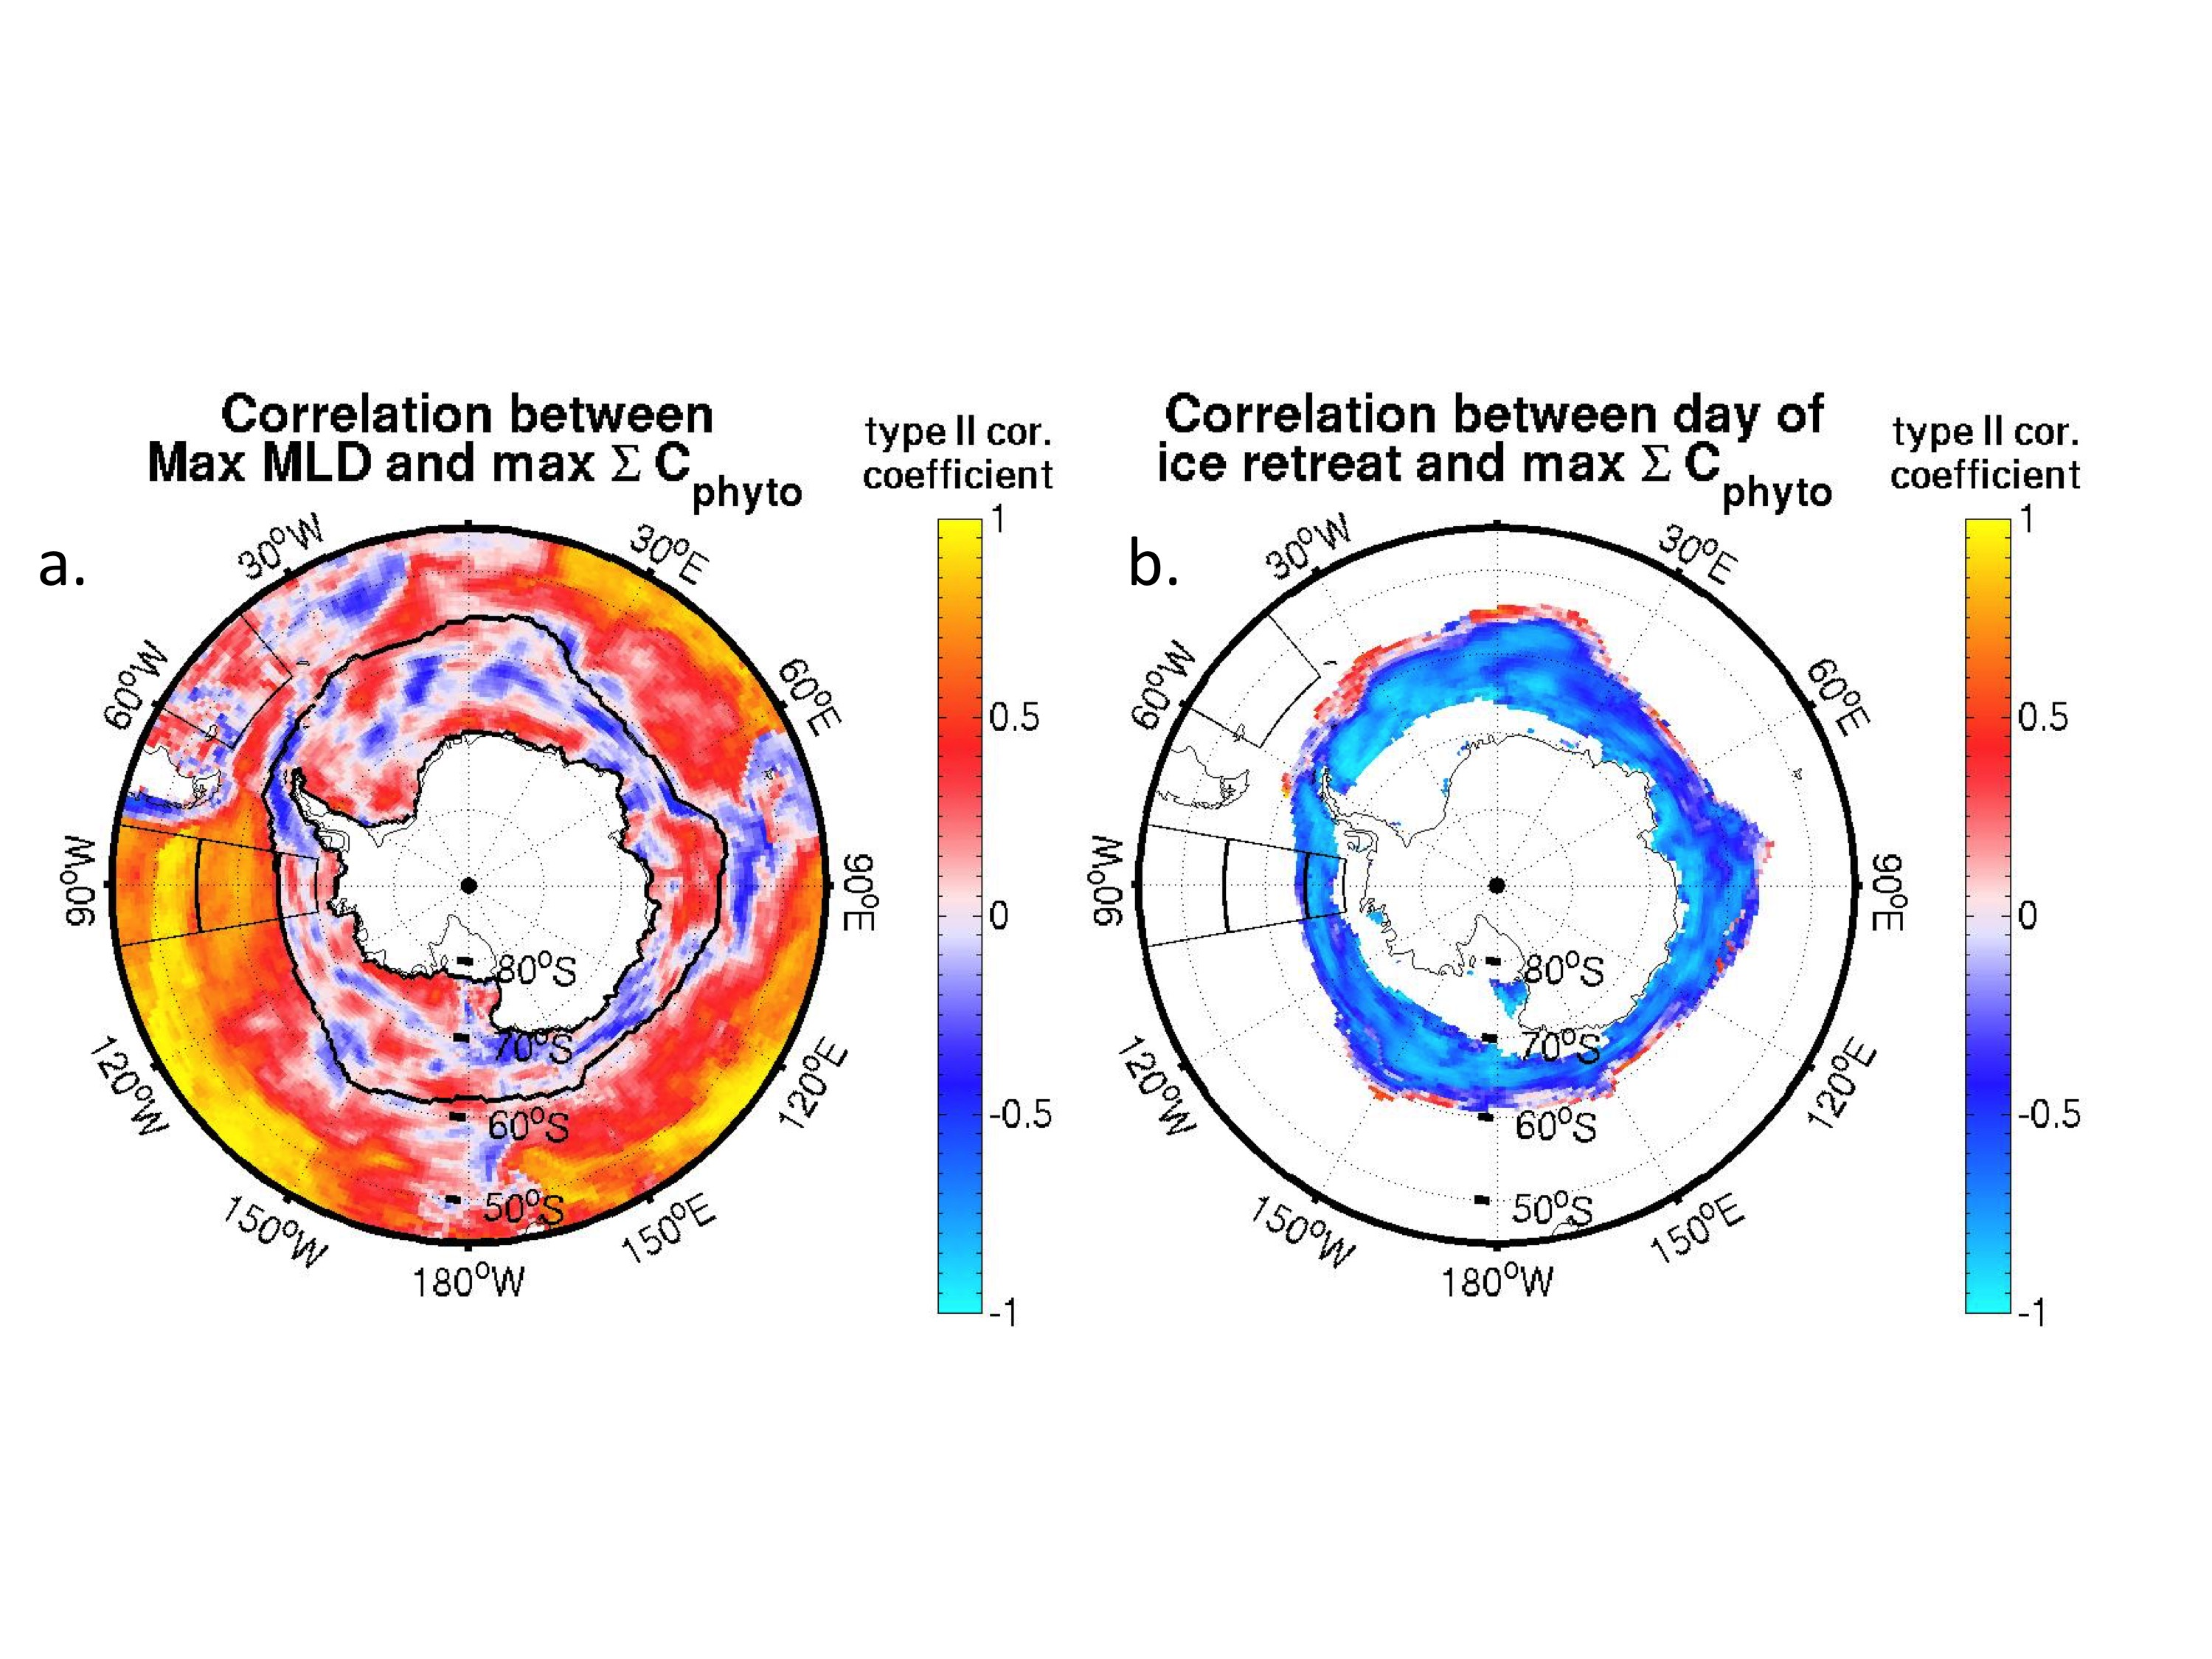
\includegraphics[scale=.18]{figures/Ch2/Figure_9.jpg}
\end{adjustwidth}
\caption[Simulated bio-physical correlations]{The simulated interannual correlation between (\textbf{a}) the maximum mixed layer depth and maximum $\Sigma C_{phyto}$ and (\textbf{b}) the day of sea-ice retreat (which co-varies with total annual ice volume) and maximum  $\Sigma C_{phyto}$ across all years of the simulation computed independently at each model grid cell. The region that sees, on average, at least 15\% mean annual fractional ice coverage is outlined in (\textbf{a}), along with regional bins P1, P2, P3, and A1 in both subplots.}
\label{fig:Fig9}
\end{figure}